\documentclass[12pt,a4paper,oneside]{report}
\usepackage{fontspec}
\setmainfont{Times New Roman}
\setsansfont{Arial}
\setmonofont{Consolas}[Scale=0.88]
\usepackage[left=2.5cm,right=2cm,top=2cm,bottom=2cm,headheight=16pt]{geometry}
\usepackage{graphicx,array,longtable,booktabs,xcolor,amsmath,float}
\usepackage{fancyhdr,titlesec,enumitem}
\usepackage[unicode,colorlinks=true,linkcolor=black,citecolor=black,urlcolor=blue]{hyperref}
\hypersetup{pdftitle={SmartRoom - Bao cao do an IoT CO3037},pdfauthor={Bui Quoc Thai; Nguyen Vinh Anh Quan}}
\definecolor{accent}{HTML}{1A5E47}
\titleformat{\chapter}[display]{\normalfont\bfseries\Large\color{accent}}{CHƯƠNG \thechapter}{8pt}{\LARGE}
\titlespacing*{\chapter}{0pt}{0pt}{20pt}
\titleformat{\section}{\normalfont\large\bfseries}{\thesection}{.7em}{}
\titleformat{\subsection}{\normalfont\normalsize\bfseries}{\thesubsection}{.7em}{}
\renewcommand{\contentsname}{MỤC LỤC}
\renewcommand{\listfigurename}{DANH MỤC HÌNH}
\renewcommand{\listtablename}{DANH MỤC BẢNG}
\renewcommand{\bibname}{TÀI LIỆU THAM KHẢO}
\renewcommand{\figurename}{Hình}
\renewcommand{\tablename}{Bảng}
\renewcommand{\chaptername}{Chương}
\setlength{\parindent}{1.1em}
\setlength{\parskip}{4pt}
\renewcommand{\baselinestretch}{1.15}
\renewcommand{\arraystretch}{1.2}
\setlength{\tabcolsep}{5pt}
\setlist{itemsep=3pt,topsep=5pt}
\setcounter{tocdepth}{2}
\setcounter{secnumdepth}{2}
\emergencystretch=3em
\pagestyle{fancy}
\fancyhf{}
\fancyhead[L]{\small CO3037 -- Internet of Things}
\fancyhead[R]{\small SmartRoom}
\fancyfoot[C]{\thepage}
\newcolumntype{P}[1]{>{\raggedright\arraybackslash}p{#1}}
% The installed MiKTeX longtable output uses infinitely shrinking \vss.
% Use stretch-only glue inside tables so page splitting remains well-defined.
\AddToHook{env/longtable/begin}{\let\vss\vfil}
\newcommand{\code}[1]{\nolinkurl{#1}}
\newcommand{\pending}{Chưa kiểm chứng}
\newcommand{\notice}[1]{\begin{quote}\small\color{accent}\textbf{Phạm vi bằng chứng.} #1\end{quote}}
\newcommand{\ClassCode}{CO3037}
\newcommand{\GroupCode}{Chưa được cấp}
\newcommand{\Instructor}{TS. Nguyễn Hòa Hưng}
\newcommand{\ReportDate}{18/11/2026}
\newcommand{\VideoLink}{Chưa cung cấp}
\newcommand{\DashboardLink}{Đã import SmartRoom CO3037 và gửi ảnh; chưa cung cấp URL dashboard}
\newcommand{\RepoURL}{https://github.com/Funacius/smartroom-iot-co3037}
\newcommand{\TestCount}{29}
\newcommand{\TestFailures}{0}
\newcommand{\AIAccuracy}{98.58}
\newcommand{\AIPrecision}{96.59}
\newcommand{\AIRecall}{99.25}
\newcommand{\AIFone}{0.9790}
\newcommand{\AITrainCount}{1500}
\newcommand{\AITestCount}{1200}
\newcommand{\MemberOneName}{Bùi Quốc Thái}
\newcommand{\MemberOneID}{2353086}
\newcommand{\MemberOneEmail}{thai.bui1569@hcmut.edu.vn}
\newcommand{\MemberTwoName}{Nguyễn Vinh Anh Quân}
\newcommand{\MemberTwoID}{2353007}
\newcommand{\MemberTwoEmail}{quan.nguyenvinhanh@hcmut.edu.vn}
\newcommand{\IngestN}{1000}
\newcommand{\IngestMean}{0.993}
\newcommand{\IngestMin}{0.697}
\newcommand{\IngestMax}{5.446}
\newcommand{\IngestPNinetyFive}{1.402}
\newcommand{\SnapshotN}{100}
\newcommand{\SnapshotMean}{0.504}
\newcommand{\SnapshotMin}{0.412}
\newcommand{\SnapshotMax}{0.842}
\newcommand{\SnapshotPNinetyFive}{0.757}
\newcommand{\InferenceN}{100}
\newcommand{\InferenceMean}{5.497}
\newcommand{\InferenceMin}{4.432}
\newcommand{\InferenceMax}{11.741}
\newcommand{\InferencePNinetyFive}{7.330}
\newcommand{\TrueNegative}{786}
\newcommand{\FalsePositive}{14}
\newcommand{\FalseNegative}{3}
\newcommand{\TruePositive}{397}


\begin{document}
\begin{titlepage}
\centering
{\bfseries ĐẠI HỌC QUỐC GIA THÀNH PHỐ HỒ CHÍ MINH\par}
{\bfseries TRƯỜNG ĐẠI HỌC BÁCH KHOA\par}
{\bfseries KHOA KHOA HỌC VÀ KỸ THUẬT MÁY TÍNH\par}
\vspace{0.9cm}

\includegraphics[width=2.8cm,height=2.8cm,keepaspectratio]{../docs/source/template-logo.png}\par
\vspace{0.8cm}
{\LARGE\bfseries BÁO CÁO ĐỒ ÁN MÔN HỌC\par}
\vspace{0.3cm}
{\Large INTERNET OF THINGS (IoT)\par}
\vspace{0.6cm}
{Học kỳ 261 -- Năm học 2026--2027\par}
\vspace{0.7cm}
{\Large\bfseries\color{accent} SMARTROOM\par}
\vspace{0.3cm}
{\Large\bfseries GIÁM SÁT MÔI TRƯỜNG PHÒNG HỌC\par}
{\Large\bfseries VÀ ĐIỀU KHIỂN QUẠT QUA COREIOT\par}
\vspace{0.8cm}
{Giảng viên hướng dẫn: \textbf{\Instructor}\par}
{Mã môn/lớp: \textbf{\ClassCode} \quad Nhóm: \textbf{\GroupCode}\par}
\vspace{0.5cm}
\small
\begin{tabular}{c P{4.6cm} c P{5.8cm}}
\toprule STT & Họ và tên & MSSV & Email \\ \midrule
1 & \MemberOneName & \MemberOneID & \MemberOneEmail \\
2 & \MemberTwoName & \MemberTwoID & \MemberTwoEmail \\
\bottomrule
\end{tabular}
\vfill
{Thành phố Hồ Chí Minh, ngày \ReportDate\par}
\end{titlepage}

\pagenumbering{roman}
\chapter*{THÔNG TIN NỘP BÀI}
\addcontentsline{toc}{chapter}{Thông tin nộp bài}
\begin{longtable}{P{4cm}P{11cm}}
\toprule Hạng mục & Thông tin \\ \midrule
GitHub & \href{\RepoURL}{github.com/Funacius/smartroom-iot-co3037} \\
Quyền truy cập & Repository riêng tư; cần cấp quyền cho giảng viên trước khi nộp. \\
Video demo & \VideoLink. Kịch bản dự kiến tại \code{docs/DEMO.md}. \\
Dashboard CoreIOT & \href{\DashboardLink}{Liên kết dashboard đã cung cấp}; cần đối chiếu với export bản đang dùng. \\
Ngày dựng báo cáo & \ReportDate; chưa xác nhận ngày nộp LMS. \\
Mã môn/lớp & \ClassCode\ (theo thông tin nhóm cung cấp). \\
Mã nhóm & \GroupCode. Tên PDF hiện dùng CHUA\_CAP\_MA\_NHOM. \\
Tài liệu gốc & \code{Project_Annoucement_IoT.pdf} và \code{IoTReport_Template.docx}. \\
\bottomrule
\end{longtable}
\notice{Cập nhật ngày 26/11/2026: web PC đã dùng switch và đồng bộ hai chiều với CoreIOT; các RPC mới có trạng thái applied. Người dùng đã thử dừng/chạy lại gateway: lệnh báo lỗi khi dừng, đồng bộ trở lại sau khởi động. Đánh giá AI bổ sung so sánh ngưỡng, năm seed mới, bất thường hiếm và dịch phân bố; model vẫn dùng dữ liệu sinh. Hai firmware đã build nhưng nhóm hiện chưa có mạch để nạp và đo phần cứng. Các ảnh/export CoreIOT gốc được giữ nguyên theo ngày thu; chưa có video và mã nhóm chính thức.}

\chapter*{BẢNG PHÂN CÔNG CÔNG VIỆC}
\addcontentsline{toc}{chapter}{Bảng phân công công việc}
Đây là \textbf{phân công đề xuất để triển khai và bảo vệ}, chưa xác nhận tỷ lệ đóng góp đã hoàn thành. Sau thử nghiệm tại lớp, nhóm cần cập nhật theo công việc và commit thực tế của từng người.
\begin{longtable}{c P{3.9cm} c P{5.8cm} c}
\toprule STT & Họ và tên & MSSV & Công việc phụ trách & Tỷ lệ \\ \midrule
1 & \MemberOneName & \MemberOneID & Firmware cảm biến/bridge; ESP-NOW (T06); web trên board (T07); lắp mạch và đo phần cứng; cùng viết Chương 2--4. & 50\% \\
2 & \MemberTwoName & \MemberTwoID & Gateway (T08), AI (T09), dashboard (T10, N06); cấu hình CoreIOT (T11--T13, T15); tổng hợp báo cáo, cùng đo và quay demo. & 50\% \\
\bottomrule
\end{longtable}
Tổng tỷ lệ đề xuất: 100\%. Cả hai thành viên phải giải thích được luồng dữ liệu và điều khiển; không tạo lịch sử Git giả cho thành viên chưa tự thực hiện commit. Phạm vi trợ giúp AI được khai báo ở phụ lục.

\chapter*{BẢNG TỰ ĐÁNH GIÁ YẾU TỐ CÔNG NGHỆ}
\addcontentsline{toc}{chapter}{Bảng tự đánh giá yếu tố công nghệ}
\noindent\textbf{Quy ước:} ``Phần mềm'' là đã chạy/kiểm thử trên PC; ``Build'' là biên dịch đạt, chưa chứng minh chạy trên board; ``Cấu hình'' là đã chuẩn bị file/hướng dẫn, chưa kiểm chứng server; ``Không'' là không triển khai. Không dùng tổng điểm mục tiêu thay cho điểm đã được công nhận.
\small
\begin{longtable}{P{.8cm}P{3.5cm}P{.95cm}P{2cm}P{1.2cm}P{4.85cm}}
\toprule Mã & Yếu tố & Điểm & Trạng thái & Mục & Bằng chứng / việc còn thiếu \\ \midrule
\endfirsthead
\toprule Mã & Yếu tố & Điểm & Trạng thái & Mục & Bằng chứng / việc còn thiếu \\ \midrule
\endhead
T01 & I2C trên Tasmota & 0,5 & Không & 2.4 & DHT20 chạy Arduino, không nhận T01. \\
T02 & Modbus RS485 & 1 & Không & 2.4 & Không có thiết bị RS485. \\
T03 & Cảm biến BLE & 1,5 & Không & 2.4 & Không dùng BLE. \\
T04 & TinyML trên board & 1 & Không & 3.5 & AI đặt trên PC, không phải TinyML. \\
T05 & Công cụ TinyML & 1 & Không & 3.5 & Không xuất model cho board. \\
T06 & ESP-NOW & 1,5 & Build & 3.3 & \code{firmware/src/main.cpp}; log build. Thiếu log hai board thực. \\
T07 & Web trên thiết bị & 1 & Build & 3.2.2 & WebServer trong firmware bridge. Thiếu ảnh/trình diễn board. \\
T08 & Gateway PC hai chiều & 1 & Phần mềm & 3.4 & Telemetry và RPC cloud mô phỏng đã chạy; thiếu USB/phần cứng thật. \\
T09 & AI trên gateway & 1 & Phần mềm & 3.5 & \code{ai_evaluation.json}; so sánh ngưỡng, dịch phân bố, test model thật; chưa có dữ liệu thực. \\
T10 & Giao diện gateway & 1 & Phần mềm & 3.4 & Switch, kiểm tra Chrome và ACK mô phỏng; đồng bộ RPC hai chiều. \\
T11 & Template CoreIOT & 1 & Phần mềm; ảnh & 3.6.1 & Hình \ref{fig:coreiot-dashboard}; export dashboard có switch, đơn vị \% đúng. \\
T12 & RuleChain & 1 & Phần mềm; ảnh & 3.6.2 & Hình \ref{fig:coreiot-root}, \ref{fig:coreiot-alarms}; hai JSON export và kiểm tra logic. \\
T13 & Gửi thông báo & 0,5 & Phần mềm; ảnh & 3.6.2 & Hình \ref{fig:coreiot-notifications}: Web notification tạo/xóa đã nhận. \\
T14 & OTA & 2 & Không & 3.6.3 & Không có OTA. \\
T15 & Đồng bộ gateway & 2 & Phần mềm & 3.4 & RPC mới applied, đồng bộ hai chiều và thử dừng/chạy lại; nguồn sensor mô phỏng. \\
\bottomrule
\end{longtable}

\begin{longtable}{P{.8cm}P{4.6cm}P{.95cm}P{2cm}P{1.2cm}P{3.75cm}}
\toprule Mã & Tính năng nâng cao & Điểm & Trạng thái & Mục & Bằng chứng \\ \midrule
N01 & Trợ lý LLM & 1 & Không & 3.7 & Không sử dụng. \\
N02 & Âm thanh/giọng nói & 1 & Không & 3.7 & Không sử dụng. \\
N03 & Màn hình LVGL & 1 & Không & 3.7 & Không sử dụng. \\
N04 & AI trên GPU thiết bị & 1 & Không & 3.7 & AI chạy CPU máy tính. \\
N05 & Ứng dụng mobile riêng & 1 & Không & 3.7 & Web responsive không tự nhận là mobile app. \\
N06 & Dashboard riêng ghi sự kiện & 1 & Phần mềm & 3.7 & Dashboard HTML, SQLite journal, CSV, kiểm tra Chrome. \\
N07 & ThingsBoard tự triển khai & 1 & Không & 3.7 & Dùng CoreIOT của lớp; không dựng server cục bộ. \\
\bottomrule
\end{longtable}
\normalsize
Tổng công nghệ \textbf{mục tiêu} của T06--T13 (trừ T14) và T15 là 10 điểm trước trần; tối đa được tính 8. N06 có mục tiêu 1 điểm. Báo cáo tối đa 2 điểm. Theo đề bài \cite{assignment}, điểm cuối là
\[
\min\!\left(10,\;\min(8,\Sigma T)+R+\min(1,\Sigma N)\right),\quad 0\leq R\leq2.
\]
Chưa chốt điểm tự nhận cho các mục phần cứng/cloud. Giảng viên đánh giá dựa trên mức hoàn thành và bằng chứng thực tế.

\tableofcontents
\listoffigures
\listoftables
\chapter*{DANH MỤC TỪ VIẾT TẮT}
\addcontentsline{toc}{chapter}{Danh mục từ viết tắt}
\begin{longtable}{P{3cm}P{12cm}}
\toprule Từ viết tắt & Ý nghĩa \\ \midrule
IoT & Internet of Things -- Internet vạn vật. \\
ESP-NOW & Giao thức truyền dữ liệu không cần kết nối Wi-Fi của Espressif. \\
I2C & Inter-Integrated Circuit -- bus nối cảm biến. \\
MQTT & Message Queuing Telemetry Transport -- giao thức pub/sub. \\
RPC & Remote Procedure Call -- lời gọi điều khiển từ xa. \\
ACK / PUBACK & Xác nhận thiết bị / xác nhận broker MQTT đã nhận bản tin. \\
TLS & Transport Layer Security -- bảo vệ kênh truyền MQTT. \\
TTL & Time to Live -- thời gian hiệu lực lệnh. \\
NVS & Non-Volatile Storage -- lưu trữ bền trên ESP32. \\
WAL & Write-Ahead Logging -- chế độ ghi nhật ký SQLite. \\
TinyML & Học máy chạy trên vi điều khiển; không triển khai trong đồ án này. \\
OTA & Over-The-Air -- cập nhật firmware qua mạng; không triển khai. \\
\bottomrule
\end{longtable}
\clearpage\pagenumbering{arabic}
\chapter{GIỚI THIỆU}
\section{Đặt vấn đề}
Một phòng học có thể cần quan sát nhiệt độ, độ ẩm và trạng thái thiết bị từ một vị trí tập trung. Nếu chỉ xem số trên cảm biến, người quản lý khó biết thời điểm bất thường đã xảy ra, kéo dài bao lâu và lệnh điều khiển có tới thiết bị hay chưa. Đồ án chọn một mô hình phòng học có một điểm đo và một quạt DC thấp áp để giải quyết ba yêu cầu: quan sát hiện tại, lưu lại sự kiện và kiểm chứng đường điều khiển.

Đây là bài toán thiết kế kỹ thuật trong phạm vi môn học; nhóm chưa khảo sát định lượng mức độ phổ biến tại trường và không đưa ra số liệu tiết kiệm điện hay cải thiện sức khỏe chưa đo. Hai đại lượng nhiệt độ/độ ẩm không đủ kết luận chất lượng không khí, nồng độ CO$_2$ hoặc hiệu quả thông gió. Ngưỡng 32~°C và 80~\%RH là tham số trình diễn có thể cấu hình, không phải giới hạn sức khỏe do dự án xác lập.

YoloUNO tích hợp ESP32-S3 và các cổng kết nối phục vụ mô hình cảm biến/điều khiển; tài liệu OhStem hướng dẫn DHT20 gắn vào cổng I2C của board \cite{ohstem}. ESP-NOW hỗ trợ trao đổi dữ liệu trực tiếp giữa ESP32 \cite{espnow}. Hai đặc điểm này phù hợp với yêu cầu nhiều thiết bị của đề bài \cite{assignment}, trong đó một board đo/điều khiển và board còn lại làm cầu nối đến PC.

\section{Các giải pháp liên quan}
Nhóm đối chiếu ba hướng triển khai từ tài liệu chính thức. Mẫu DHT20 của OhStem là cơ sở xác định vai trò và cách nối cảm biến \cite{ohstem}; thư viện DHT20 cung cấp API đọc và mã lỗi \cite{dht20}. Dashboard Thermostats của ThingsBoard cung cấp widget giám sát có sẵn, được tái sử dụng có ghi nguồn \cite{tbtemplate}. Gateway API mô tả cách đại diện nhiều thiết bị con bằng một kết nối MQTT \cite{gatewayapi}. Isolation Forest là lựa chọn thuật toán phát hiện điểm dữ liệu khác biệt với phân bố huấn luyện \cite{isolation}.

\begin{table}[H]\centering\small
\caption{So sánh các hướng triển khai trong phạm vi đồ án}
\begin{tabular}{P{3cm}P{4.2cm}P{3.8cm}P{3.6cm}}
\toprule Hướng & Điểm phù hợp & Hạn chế trong phạm vi chọn & Cách dùng trong SmartRoom \\ \midrule
Hiển thị DHT20 tại chỗ & Dễ lắp, dễ kiểm tra số đo & Cần bổ sung lưu sự kiện và điều khiển xa & Kế thừa nguyên lý đọc cảm biến \\
Node kết nối cloud trực tiếp & Ít tầng trung gian & Mỗi node cần kết nối/token; thiếu PC phân tích cục bộ & Không chọn cho luồng chính \\
Gateway + dashboard template & Gom dữ liệu và RPC của child; có widget có sẵn & Phải xử lý mất mạng và đồng bộ & Chọn, bổ sung SQLite/ACK/AI \\
\bottomrule
\end{tabular}
\end{table}

Khoảng trống nhóm tập trung là làm rõ sự khác nhau giữa ``đã gửi lệnh'', ``broker đã nhận'' và ``node đã áp dụng'', đồng thời cung cấp minh chứng lặp lại được. SmartRoom không tuyên bố vượt trội sản phẩm thương mại; phần đóng góp nằm ở cách tích hợp các khối và cơ chế đánh giá minh bạch.

\section{Mục tiêu dự án}
Mục tiêu tổng quát là xây dựng mô hình IoT hai board có đường thu thập và điều khiển hai chiều, kết nối CoreIOT, dễ đọc mã nguồn và dễ trình bày khi bảo vệ. Các mục tiêu kiểm chứng được chia theo điều kiện đo:
\begin{enumerate}
\item Cứ 2 giây lấy mẫu DHT20; dữ liệu lỗi không được thay bằng giá trị giả. Cần kiểm tra trên board thật.
\item Dữ liệu được lưu bền và hiển thị ở PC; sau hơn 15 giây không có mẫu mới phải báo stale, giữ số liệu cuối để truy vết.
\item Lệnh có TTL 5 giây, retry 0,5 giây; chỉ xác nhận áp dụng khi nhận ACK đúng ID và giá trị. Khi mất xác nhận phải ghi thất bại và trạng thái vật lý chưa rõ.
\item Giữ nguyên 1.000 bản tin đã lưu khi publish thất bại và khởi động lại; xóa outbox sau xác nhận từ transport. Đây là kiểm thử phần mềm, không phải phép đo Internet.
\item Xây quy trình AI không dùng tập test để huấn luyện; xuất confusion matrix và thời gian suy luận trên CPU. Chỉ đánh giá khả năng triển khai thực sau khi có dữ liệu thật.
\item Trên hệ thống thực, đặt mục tiêu sensor tới dashboard dưới 5 giây và lệnh tới ACK dưới 2 giây trong điều kiện phòng lab; hiện chưa có phép đo để xác nhận hai mục tiêu này.
\end{enumerate}

\section{Các tính năng đề xuất}
\begin{longtable}{P{1cm}P{8.2cm}P{3.1cm}P{2cm}}
\caption{Danh sách tính năng có thể kiểm chứng}\label{tab:features}\\
\toprule Mã & Mô tả & Thiết bị thực hiện & Ưu tiên \\ \midrule
F01 & Đo nhiệt độ/độ ẩm mỗi 2 giây; gửi gói có boot ID và sequence qua ESP-NOW. & Node A, node B & Bắt buộc \\
F02 & Lưu SQLite, hiển thị giá trị/biểu đồ; phát hiện dữ liệu cũ sau 15 giây. & PC gateway & Bắt buộc \\
F03 & Phát hiện vượt ngưỡng với hysteresis và ghi sự kiện raised/cleared. & PC, CoreIOT & Bắt buộc \\
F04 & Suy luận bất thường từ hai đại lượng; ghi score và thời gian suy luận. & PC gateway & Nâng cao \\
F05 & Bật/tắt quạt từ dashboard PC hoặc web bridge; theo dõi pending/applied/failed bằng ACK node. & PC, hai board & Bắt buộc \\
F06 & Đồng bộ child, gửi telemetry, nhận/trả RPC CoreIOT; phát lại dữ liệu lưu khi nối lại. & PC, CoreIOT & Bắt buộc \\
F07 & Xem dashboard từ template, tạo/xóa alarm bằng RuleChain và gửi notification khi tạo alarm. & CoreIOT & Bắt buộc \\
F08 & Xuất CSV sự kiện và tái hiện kiểm thử theo kịch bản có log/biểu đồ. & PC gateway & Bắt buộc \\
\bottomrule
\end{longtable}

F03 và F04 là hai cơ chế tách biệt: luật ngưỡng dễ giải thích, còn AI nhận diện độ khác biệt với dữ liệu huấn luyện. Đầu ra AI không trực tiếp tự bật quạt trong phiên bản này. Điều khiển bằng tay giúp tách việc đánh giá mô hình khỏi việc đánh giá cơ cấu chấp hành.

\section{Phạm vi và giới hạn}
Mô hình triển khai dự kiến gồm hai YoloUNO, một DHT20, một bộ driver/quạt và một PC. Chưa xét cấp nguồn pin, công suất tiêu thụ, độ bền 24 giờ, mạng nhiều phòng hoặc chứng nhận an toàn. Không dùng RS485, BLE, Tasmota, TinyML, OTA hay ứng dụng di động native.

Tại ngày 26/11/2026, nhóm đã build firmware, chạy gateway mô phỏng, đồng bộ switch web--CoreIOT hai chiều và đánh giá AI trên dữ liệu sinh. Người dùng xác nhận dừng/chạy lại gateway khôi phục đồng bộ; chưa có phép đo thời gian phục hồi. Nhóm hiện chưa có mạch nên chưa nạp firmware hoặc đo cảm biến/radio. Hình wiring là bản đề xuất; ảnh ứng dụng và log cloud dùng nguồn mô phỏng. Các giới hạn này được giữ rõ trong bảng tự đánh giá.

\section{Cấu trúc báo cáo}
Chương 2 ánh xạ tính năng vào kiến trúc, phần cứng và mã chấm điểm. Chương 3 mô tả firmware, gateway, AI và cấu hình cloud. Chương 4 nêu cách đo, kết quả đã chạy và các phép đo cần bổ sung. Chương 5 tổng kết mức hoàn thành và hướng phát triển. Chương 6 hướng dẫn cài, cấu hình, build, nạp và vận hành mã nguồn. Phụ lục ghi nguồn minh chứng, kịch bản demo và phạm vi dùng AI.

\chapter{PHÂN TÍCH HỆ THỐNG}
\section{Kiến trúc tổng thể}
Hệ thống chọn mô hình IoT Gateway. Node A đọc DHT20 và điều khiển driver quạt; node B chuyển tiếp ESP-NOW/USB và cung cấp web cục bộ. PC tổng hợp, lưu bền, suy luận và kết nối CoreIOT. Trên cloud, sensor được đại diện bằng child device \code{room-node-01}, qua gateway \code{smartroom-pc-gateway}.
\begin{figure}[H]\centering
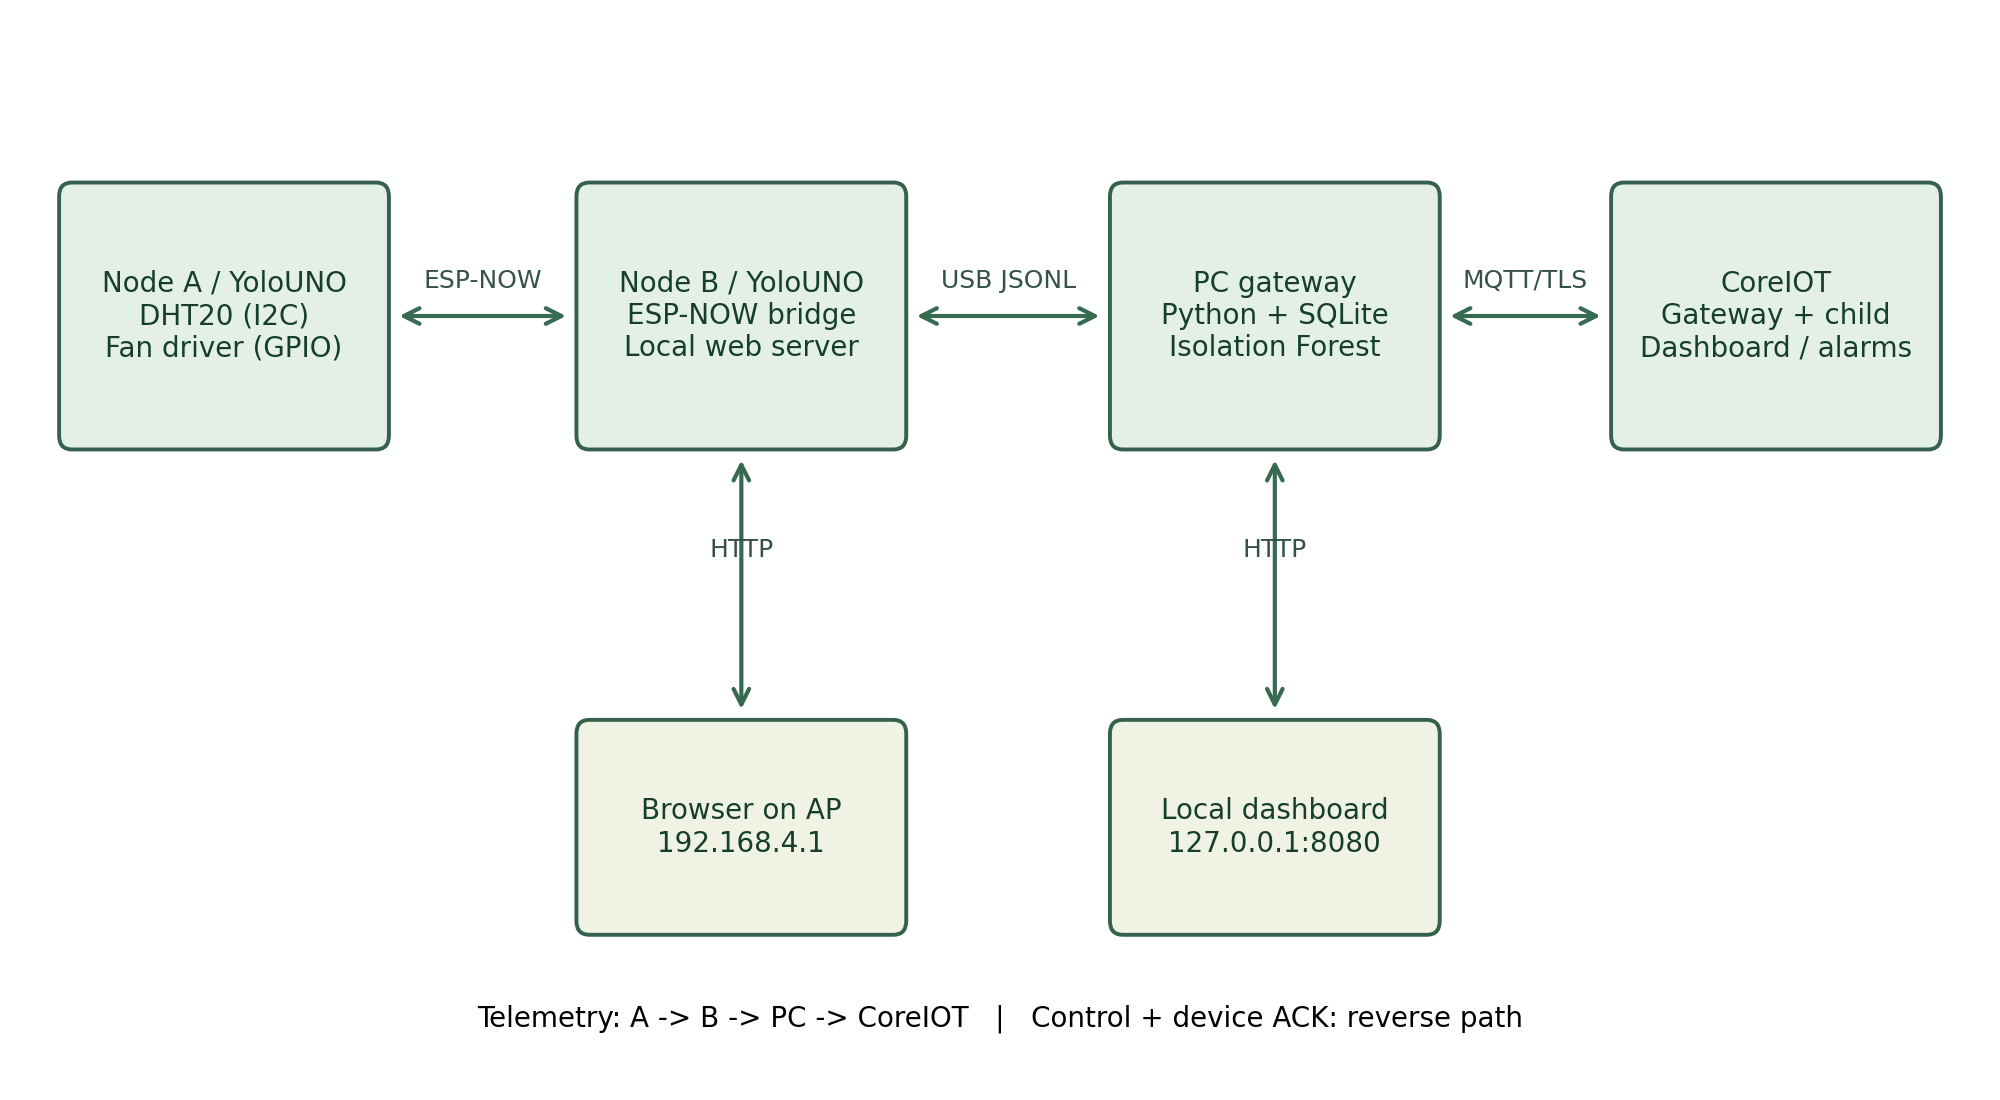
\includegraphics[width=\textwidth]{figures/architecture.png}
\caption{Kiến trúc thiết kế; mũi tên hai chiều thể hiện telemetry và điều khiển/ACK.}
\end{figure}
PC giúp cô lập phần kết nối cloud và AI khỏi firmware. USB Serial được chọn giữa bridge và PC để không bắt board vừa tham gia Wi-Fi Internet vừa đổi channel của ESP-NOW. PC có thể dùng Wi-Fi hoặc Ethernet riêng để ra Internet. Khi kiểm tra web bridge, người dùng có thể dùng điện thoại kết nối AP; nếu PC đổi sang AP bridge và mất Internet thì cloud tạm ngắt, outbox vẫn lưu dữ liệu.

\section{Phân rã chức năng}
Thu thập gồm đọc, kiểm tra mã lỗi, đóng gói, truyền và giải mã. Giám sát gồm kiểm tra cấu trúc, loại trùng, lưu đọc gần nhất và hiển thị. Phát hiện sự kiện gồm ngưỡng, hysteresis, AI và ghi journal. Điều khiển gồm kiểm tra tham số, cấp ID, retry, áp dụng GPIO, ACK và trả kết quả cho nguồn yêu cầu.
\begin{figure}[H]\centering
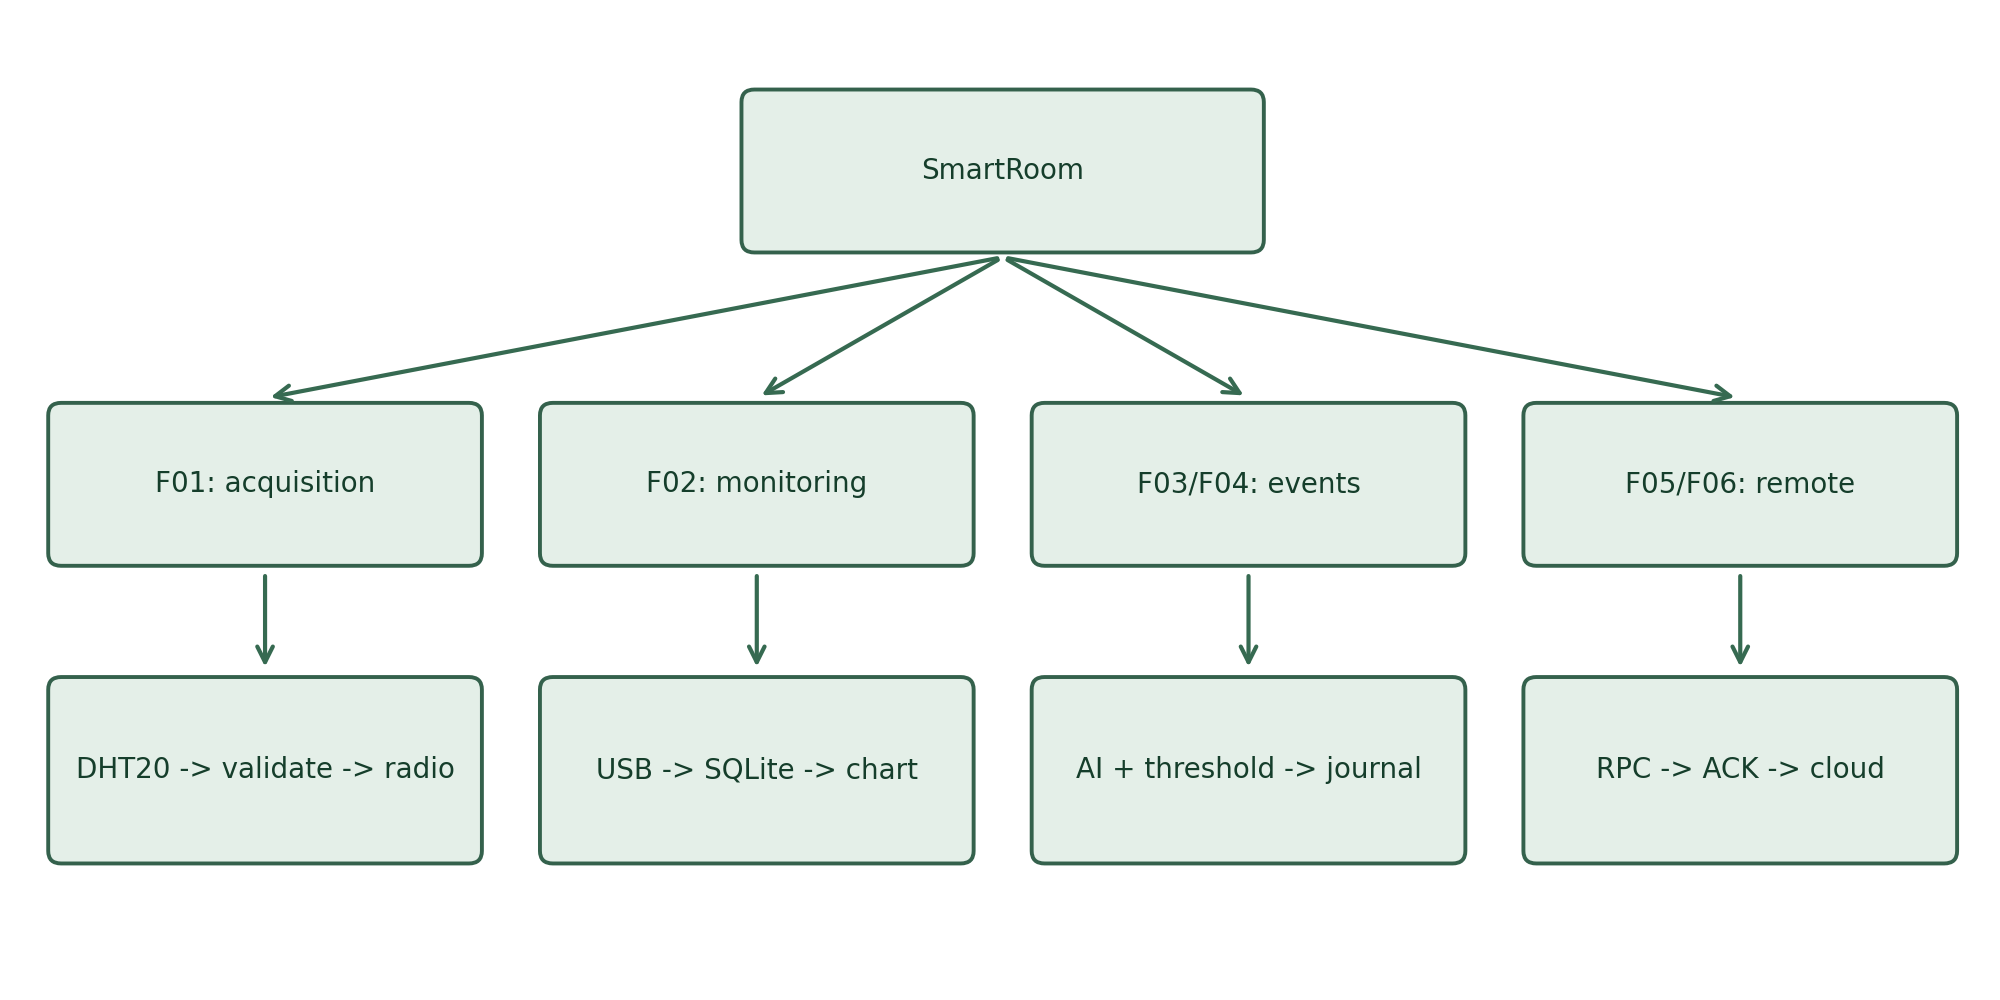
\includegraphics[width=\textwidth]{figures/decomposition.png}
\caption{Phân rã các chức năng chính của SmartRoom.}
\end{figure}

\section{Các lớp tính năng}
\subsection{Lớp cảm biến}
DHT20 được chọn vì có hai đại lượng trên cùng bus I2C và tài liệu kết nối YoloUNO \cite{ohstem}. Thư viện được ghim phiên bản và firmware kiểm tra kết quả \code{read()} trước khi truyền. Chu kỳ 2 giây phục vụ demo và không phải chế độ tối ưu năng lượng. Sai số thực nghiệm chưa đo với thiết bị tham chiếu; báo cáo không biến thông số nhà sản xuất thành sai số thực đã chứng minh.

T01 không được đăng ký vì đề bài yêu cầu cảm biến I2C \emph{trên Tasmota}. Việc sử dụng I2C trong Arduino không đáp ứng điều kiện đó. Đây là khác biệt cần nêu rõ khi ánh xạ tiêu chí.

\subsection{Lớp truyền thông}
ESP-NOW phục vụ liên kết node A--B, ánh xạ T06. Theo Espressif, peer cần được đăng ký và hai thiết bị phải ở channel thích hợp; khóa LMK bảo vệ unicast khi mã hóa được bật \cite{espnow}. Dự án cấu hình peer MAC tĩnh, channel 1 và key 16 byte phải thay khi triển khai. Khung riêng 25 byte nằm dưới giới hạn 250 byte của phiên bản ESP-NOW dùng trong build.

Gói có magic, version, type, boot, seq, command ID, nhiệt độ, độ ẩm và trạng thái fan. MAC nguồn được lọc; header và kích thước được kiểm tra. Telemetry không có retry ở tầng ứng dụng; mất gói cần đo bằng khoảng sequence theo từng boot. Lệnh được PC retry cùng ID để node không thực hiện lặp tác động.

USB dùng JSON một dòng một bản tin (JSONL). MQTT dùng QoS 1; token là của gateway. Mã hỗ trợ TLS với kiểm chứng CA hệ thống khi server cung cấp endpoint phù hợp. Với server lớp \code{app.coreiot.io}, profile riêng dùng cổng 1883 không TLS theo tài liệu chính thức \cite{coreiotconnect}. Paho cung cấp vòng lặp mạng và thông tin xác nhận publish \cite{paho}. Xác nhận broker không chứng minh cơ cấu vật lý đã chạy.

\subsection{Lớp IoT Gateway}
PC được chọn thay vì Raspberry Pi để tận dụng máy học tập sẵn có. Module xử lý không phụ thuộc Serial/MQTT nên có thể kiểm tra bằng clock và transport giả. SQLite lưu readings, events, commands và outbox. Một giao dịch lưu reading cùng bản tin chờ gửi tránh trường hợp có dữ liệu hiển thị nhưng không có bản tin để phát lại sau khởi động.

T08 bao gồm nhận dữ liệu và phân phối điều khiển hai chiều, không chỉ upload telemetry. T10 là HTTP dashboard tại loopback. T15 là tương tác với gateway/child trên CoreIOT: connect trước telemetry, re-register khi nối lại, nhận RPC có tên child và trả đúng request ID.

\subsection{Lớp trí tuệ nhân tạo}
Bài toán là phát hiện bất thường hai biến tại PC (T09). So với việc đưa TinyML lên board, hướng này dễ theo dõi dữ liệu, thay model và đo hiệu năng cho nhóm hai người. Isolation Forest được huấn luyện từ mẫu bình thường; \code{decision_function < 0} được xem là bất thường theo API thư viện \cite{isolation}.

Không dùng GPU và không đăng ký T04, T05 hoặc N04. Bộ dữ liệu mặc định được sinh có seed; dữ liệu thật có thể nhập CSV. Việc tách tập trước khi huấn luyện là yêu cầu phương pháp: không dùng nhãn/tập test để tạo hoặc điều chỉnh model. Kết quả từ dữ liệu sinh chỉ cho thấy pipeline hoạt động theo giả thiết sinh dữ liệu.

\subsection{Lớp ứng dụng và nền tảng CoreIOT}
Ứng dụng local do dự án viết hiển thị lịch sử, tuổi bản tin, AI, outbox và journal. N06 tập trung vào phát hiện và ghi sự kiện lâu dài; không tự nhận N05 chỉ vì giao diện co giãn trên điện thoại.

CoreIOT được chuẩn bị dashboard dựa trên template (T11), RuleChain (T12), hướng dẫn notification (T13) và adapter Gateway API (T15). Alarm và notification là hai chức năng khác nhau: alarm có bản ghi trạng thái; notification phải thực sự đến recipient. Rule engine cho phép nối các node xử lý theo quan hệ đầu ra \cite{ruleengine}.

\section{Ánh xạ tính năng -- yếu tố công nghệ}
\begin{table}[H]\centering\small
\caption{Ánh xạ tính năng với danh sách chấm điểm}
\begin{tabular}{P{1.1cm}P{5.8cm}P{3.3cm}P{4.3cm}}
\toprule Tính năng & Vai trò & Mã công nghệ & Khối thực hiện \\ \midrule
F01 & Cảm biến gửi dữ liệu không dây & T06 & Node A $\rightarrow$ B \\
F02 & Tổng hợp và giám sát local & T08, T10 & PC gateway \\
F03 & Phát hiện/ghi cảnh báo; xử lý cloud & T12, T13, N06 & PC và CoreIOT \\
F04 & Phân tích AI trên gateway & T09 & PC CPU \\
F05 & Điều khiển có ACK, web trên board & T07, T08, T10 & Hai board và PC \\
F06 & Telemetry/RPC theo child qua gateway & T08, T15 & PC và CoreIOT \\
F07 & Giao diện template và RuleChain & T11, T12, T13 & CoreIOT \\
F08 & Journal sự kiện và xuất CSV & T10, N06 & Dashboard/SQLite \\
\bottomrule
\end{tabular}
\end{table}
Các mã không chọn được liệt kê rõ trong bảng tự đánh giá ở đầu báo cáo. Cách chọn ưu tiên luồng demo thống nhất thay vì ghép nhiều giao thức không phục vụ vấn đề đã nêu.

\section{Công nghệ ngoài danh sách}
SQLite, HTTP/JSONL và thư viện Python là công cụ triển khai, không được cộng điểm công nghệ độc lập. SQLite cung cấp lưu trữ giao dịch và WAL, phù hợp outbox trên một máy tính \cite{sqlite}. HTTP giúp trình duyệt đọc trạng thái; JSONL giúp phân tách bản tin Serial có thể bị chia thành nhiều lần đọc. Joblib được dùng lưu model do dự án huấn luyện; chỉ nạp file tin cậy vì định dạng này có thể thực thi khi deserialize.

\section{Danh sách phần cứng}
\begin{table}[H]\centering\small
\caption{Cấu hình phần cứng dự kiến cần lấy tại lớp}
\begin{tabular}{c P{4.5cm}P{2.9cm}c P{5.6cm}}
\toprule STT & Thành phần & Giao tiếp & SL & Vai trò / điều kiện \\ \midrule
1 & YoloUNO ESP32-S3 & I2C/GPIO/ESP-NOW & 2 & Một sensor/actuator, một bridge; xác nhận revision/pinout. \\
2 & Module DHT20 & I2C & 1 & Đo nhiệt độ/độ ẩm; đối chiếu nguồn cấp và pull-up module. \\
3 & Quạt DC thấp áp và driver & GPIO vào driver & 1 bộ & Driver tương thích logic 3,3 V; không cấp tải từ GPIO. \\
4 & Cáp USB dữ liệu & USB CDC & 2 & Nạp và nối bridge; đóng monitor trước khi gateway mở cổng. \\
5 & Máy tính có Internet & USB + mạng & 1 & Python, SQLite, AI, MQTT/TLS và HTTP. \\
\bottomrule
\end{tabular}
\end{table}
Chưa chốt chi phí vì phần cứng dùng từ lớp và chưa xác nhận danh mục module thực tế. Dự án không yêu cầu mua thêm thiết bị chỉ để tăng số lượng mã chấm điểm.

\chapter{HIỆN THỰC HỆ THỐNG}
\section{Phần cứng và sơ đồ nối dây}
\begin{figure}[H]\centering
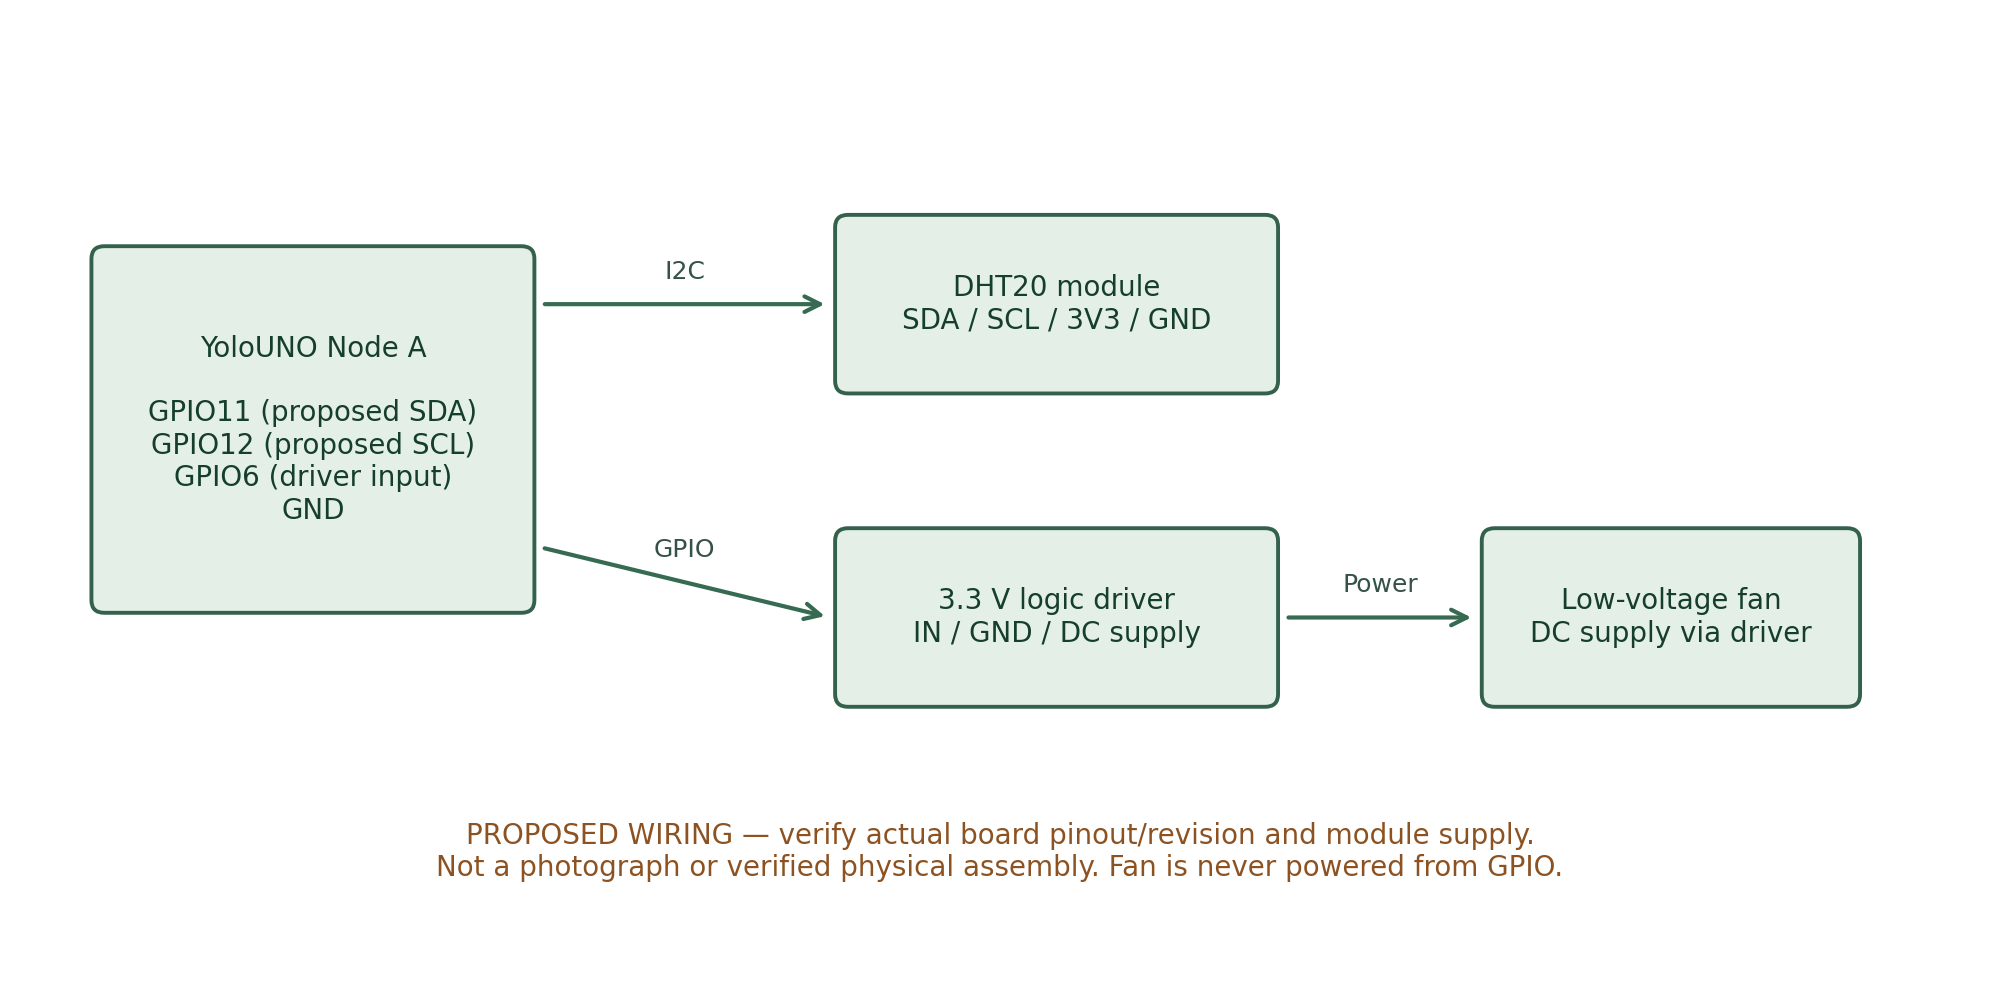
\includegraphics[width=\textwidth]{figures/wiring_proposed.png}
\caption{Sơ đồ nối dây đề xuất, chưa phải ảnh mạch đã lắp.}
\end{figure}
Chân đề xuất là GPIO11 cho SDA, GPIO12 cho SCL và GPIO6 cho tín hiệu driver. Các số này là GPIO thô của ESP32, không tự đồng nhất với nhãn D11/D12/D6 trên board. Trước khi nạp phải đối chiếu sơ đồ board thực tế, cổng I2C và thông số module. Đầu vào driver cần nhận mức logic 3,3~V; nguồn tải quạt cấp qua driver và mass tham chiếu theo module.

Board definition \code{firmware/boards/yolo_uno.json} là cấu hình build riêng của dự án: ESP32-S3, 240~MHz, flash 4~MB, DIO, không bật PSRAM và dùng variant generic với GPIO khai báo tường minh. Đây không phải khẳng định mọi phiên bản YoloUNO đều có cùng dung lượng flash. Mục đích là build trong cấu hình bộ nhớ bảo thủ; xác nhận revision và khả năng boot vẫn cần board thật.

\section{Firmware thiết bị}
\subsection{Node cảm biến/điều khiển và bridge (T06)}
Firmware dùng chung \code{main.cpp} với hai environment PlatformIO: \code{sensor} đặt \code{ROLE_SENSOR=1}, \code{bridge} đặt bằng 0. Ghim \code{espressif32@6.13.0}, Arduino-ESP32 2.0.17, ArduinoJson 6.21.5 và DHT20 0.3.2 để callback ESP-NOW và API không đổi ngoài dự kiến. Hai firmware đã build thành công; log ở \code{evidence/firmware_build.log}.

Sau boot, node đưa đầu ra quạt về tắt, tạo boot ID ngẫu nhiên, khởi tạo Wi-Fi/ESP-NOW, thêm peer với MAC và khóa cấu hình. Node sensor mở I2C, đọc DHT20 mỗi 2 giây. Chỉ khi mã trả về thành công mới đóng gói telemetry; khi lỗi, dừng phát mẫu đó và đưa đầu ra về tắt. Không thay một lần đọc lỗi bằng số 0 hoặc giá trị được sinh.

Bridge giải mã gói nhận và xuất Serial JSONL. Callback Wi-Fi chỉ kiểm tra MAC/độ dài/header rồi đẩy vào hàng đợi FreeRTOS tối đa 12 gói; JSON, Serial, ghi NVS và xử lý web nằm trong loop. Nếu hàng đợi đầy, gói có thể bị bỏ; sequence giúp nhận diện tình huống này trong phép đo thực.

Lệnh quạt dùng \emph{set trạng thái}, không dùng toggle. Node ghi command ID cuối vào NVS; ID lặp chỉ được ACK trạng thái đầu ra hiện tại, không áp dụng lại lệnh. Nếu bật quạt, lệnh có lease 30 giây rồi firmware tự đưa đầu ra về tắt. Telemetry tiếp theo công bố trạng thái mới. Khi lỗi cảm biến, đầu ra cũng tắt. Đây là chính sách của mô hình DC thí nghiệm, chưa phải chiến lược điều khiển thông gió hoàn chỉnh.

\subsection{Web server trên thiết bị (T07)}
Bridge chạy \code{WebServer} cổng 80, tạo AP \code{SmartRoom-Bridge}. Sau khi kết nối AP, trình duyệt mở \code{192.168.4.1}; trang tự viết lấy dữ liệu từ \code{/api/state}, hiển thị nhiệt độ, độ ẩm, fan và tuổi dữ liệu. API \code{/api/fan} nhận boolean và gửi \code{local_command} qua USB tới PC để dùng cùng cơ chế cấp ID/retry/ACK. Vì vậy điều khiển từ web bridge yêu cầu PC gateway đang chạy; trang vẫn xem được dữ liệu radio nếu PC ngừng.

Trang yêu cầu Basic Auth; mật khẩu AP, mật khẩu quản trị và khóa radio mẫu phải thay trong cấu hình local. Basic Auth trên HTTP không thay thế HTTPS; cấu hình này chỉ phục vụ mạng AP lab riêng. Hiện có bằng chứng build, chưa có screenshot web chạy trên board nên chưa nhận T07 hoàn tất.

\section{Truyền thông giữa các thiết bị}
\begin{table}[H]\centering\small
\caption{Khung ESP-NOW phiên bản 1, tổng cộng 25 byte}
\begin{tabular}{P{4cm}P{2.3cm}P{8cm}}
\toprule Trường & Số byte & Ý nghĩa \\ \midrule
magic, version, type & 2 + 1 + 1 & Nhận diện giao thức; telemetry/command/ACK. \\
boot, seq & 4 + 4 & Phiên khởi động và số thứ tự telemetry. \\
commandId & 4 & ID bền từ PC; đi qua bridge không thay đổi. \\
temperature, humidity & 4 + 4 & Số thực float hai đại lượng. \\
fan & 1 & Boolean mã hóa thành 0/1. \\
\bottomrule
\end{tabular}
\end{table}
Hai board cùng kiến trúc ESP32-S3 nên khung packed dùng định dạng little-endian hiện tại. Nếu bổ sung nền tảng khác cần serialization độc lập endian. Chống trùng tại PC dùng \code{(device,boot,seq)}; trong cùng boot, sequence không tăng sẽ bị bỏ. Boot ID ngẫu nhiên 32 bit có xác suất va chạm, và sequence 32 bit có thể wrap sau thời gian rất dài; phiên bản hiện tại chưa xử lý các trường hợp biên này thành giao thức tổng quát.

Ví dụ telemetry từ USB:
\begin{verbatim}
{"type":"telemetry","device":"room-node-01",
 "boot":1234,"seq":8,"temperature":27.6,
 "humidity":61.2,"fan":false}
\end{verbatim}
Gateway chấp nhận một dòng bị chia nhiều lần đọc Serial, bỏ log boot không phải JSON, từ chối object sai cấu trúc và giới hạn buffer. Giới hạn vật lý và tỷ lệ mất gói ESP-NOW chưa được đo. Bằng chứng cần bổ sung là log đồng thời ở hai board với cùng boot/seq và các phép đo khoảng cách, không phải ảnh build.

\section{IoT Gateway}
\subsection{Thu thập, lưu trữ và đường điều khiển (T08, T15)}
\code{gateway/core.py} chứa logic, \code{transports.py} chứa adapter Serial/mô phỏng/MQTT và \code{server.py} cung cấp HTTP. Khi nhận mẫu, gateway kiểm tra tên thiết bị, boot/seq kiểu integer, fan kiểu boolean, nhiệt độ hữu hạn trong $[-40,85]$ và độ ẩm trong $[0,100]$. Miền chấp nhận là hàng rào dữ liệu đầu vào, không phải sai số hay giới hạn đo đã thực nghiệm của cảm biến.

Bảng readings lưu mẫu; events lưu chuyển trạng thái; commands lưu yêu cầu điều khiển; outbox lưu topic/payload cần gửi. Ngưỡng và AI được tính trước khi lưu reading + event + outbox trong cùng giao dịch. Khi outbox đủ 100.000 bản tin, mẫu mới bị từ chối và báo lỗi thay vì âm thầm xóa dữ liệu chưa gửi. Đây là giới hạn theo số bản tin, chưa phải hạn mức tổng dung lượng đĩa.

Khi cloud nối lại, adapter đăng ký child bằng \code{v1/gateway/connect} trước khi flush telemetry. Topic, cấu trúc và tên child được triển khai theo Gateway API chuẩn \cite{gatewayapi}. Người dùng đã xác nhận Latest telemetry và nút RPC; gateway ghi các command có RPC ID và trạng thái applied với node mô phỏng. Bản tin telemetry có dạng:
\begin{verbatim}
Topic: v1/gateway/telemetry
{"room-node-01":[{"ts":1795000000000,"values":{
  "temperature":27.6,"humidity":61.2,"fan":false,
  "anomaly":false,"threshold_alarm":false,
  "data_source":"hardware"}}]}
\end{verbatim}
Timestamp là thời gian PC nhận, không phải thời điểm cảm biến lấy mẫu đã đồng bộ clock. Vì vậy không thể suy ra độ trễ radio hoặc end-to-end từ phép trừ timestamp không cùng hệ quy chiếu.

Outbox chỉ xóa sau khi Paho báo PUBACK QoS 1. Nếu broker đã nhận và PC tắt trước khi xóa, bản tin có thể gửi lại; hệ thống có ngữ nghĩa \emph{at least once}. PUBACK không xác nhận RuleChain hoặc widget đã cập nhật. Hiện readings/events chưa có chính sách lưu trữ cuốn chiếu nên cần theo dõi ổ đĩa khi chạy lâu.

RPC nhận từ cloud có dạng:
\begin{verbatim}
{"device":"room-node-01","data":{
  "id":14,"method":"setFan","params":true}}
\end{verbatim}
Gateway ghi pending và ánh xạ request ID cloud vào command ID local bền. Chỉ khi nhận ACK đúng ID/giá trị mới gửi:
\begin{verbatim}
Topic: v1/gateway/rpc
{"device":"room-node-01","id":14,
 "data":{"success":true,"fan":true,"detail":"Device ACK"}}
\end{verbatim}
\begin{figure}[H]\centering
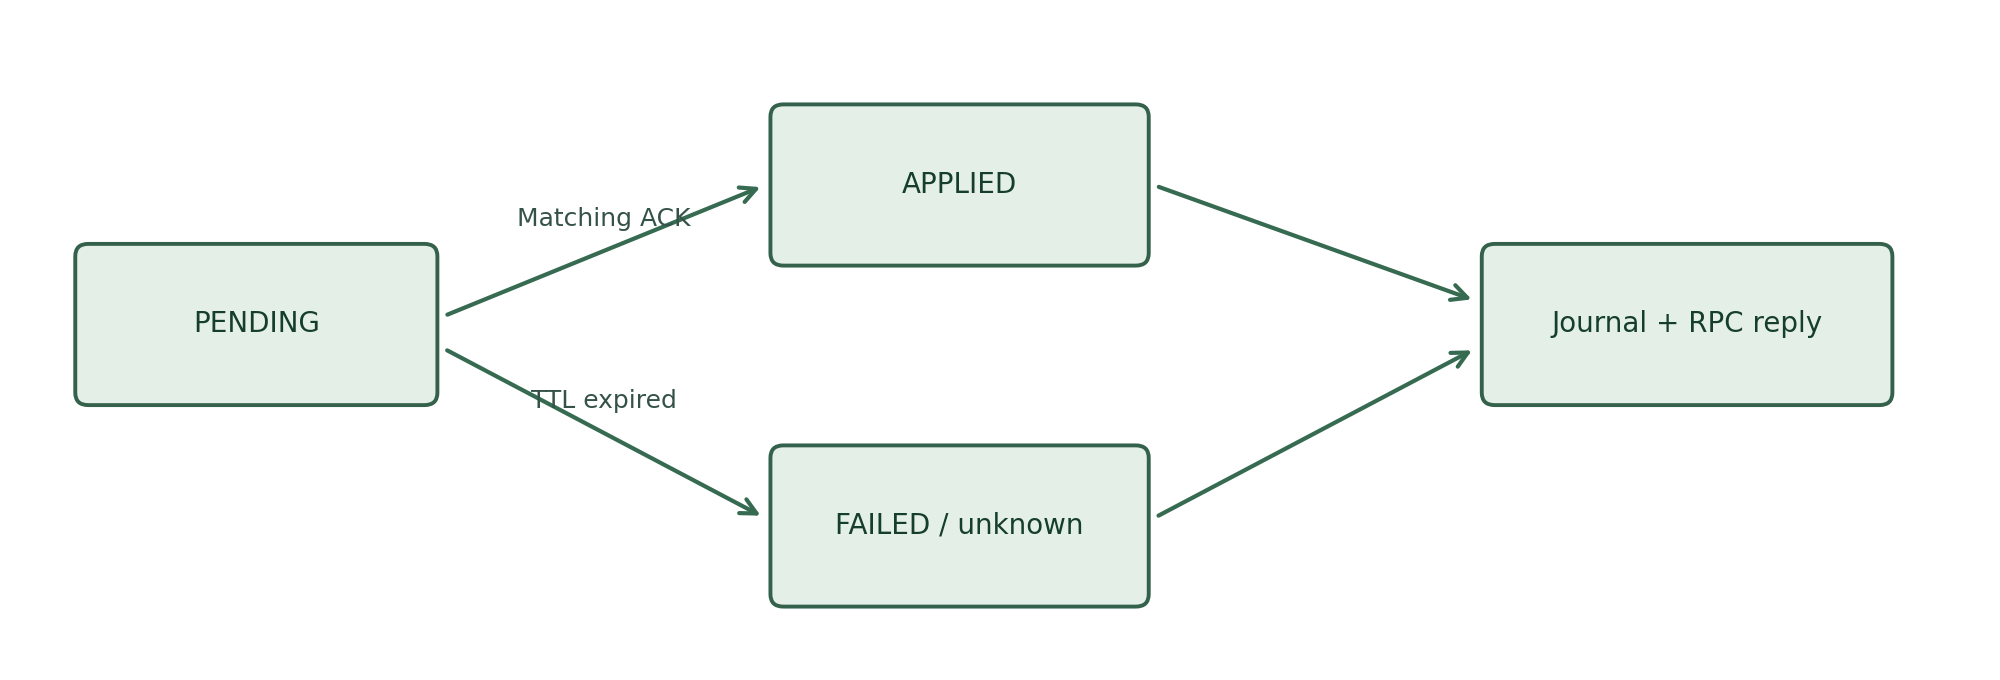
\includegraphics[width=\textwidth]{figures/command_state.png}
\caption{Lệnh hoàn thành bằng ACK; hết TTL không suy diễn trạng thái vật lý.}
\end{figure}
Mỗi thời điểm chỉ cho một lệnh pending để tránh retry bật/tắt đến đảo thứ tự. Trường hợp hết TTL được ghi failed; ACK đến muộn không đổi thành applied. Trạng thái thực tế vẫn theo telemetry, vì ACK có thể mất sau khi GPIO đã đổi. ACK xác nhận trạng thái đầu ra do firmware báo, chưa đo dòng điện hoặc tốc độ quạt.

Trong lần kiểm tra ngày 26/11, request ID RPC được dùng lại nhưng SQLite còn lệnh từ phiên cũ, khiến lệnh mới bị coi là lặp hoặc khác tham số. Bản sửa thêm phạm vi phiên MQTT vào khóa chống lặp; mỗi kết nối thành công có session ID riêng. ID lệnh local gửi xuống node vẫn tăng và lưu bền. Test kiểm tra cả lệnh cùng/khác giá trị giữa hai phiên và lệnh lặp trong cùng phiên. Sau khi khởi động lại bản sửa, người dùng xác nhận web--CoreIOT đồng bộ hai chiều; API gateway ghi các RPC ID 4, 5, 6 tương ứng lệnh 18, 19, 20 đều applied. Minh chứng nằm ở \code{evidence/fan_sync_live_check.json}; sensor vẫn mô phỏng.

\subsection{Giao diện giám sát và điều khiển (T10)}
HTTP server mặc định chỉ bind \code{127.0.0.1}. API \code{/api/state} trả reading mới nhất, 120 mẫu gần nhất, 60 sự kiện gần nhất, 20 lệnh gần nhất và số outbox. Sau 15 giây không có mẫu mới, trạng thái hiển thị stale. Dashboard dùng một switch bật/tắt và phân biệt pending/applied/failed. Switch cập nhật từ telemetry hoặc ACK mới hơn bản tin gần nhất, tạm khóa khi chờ xác nhận hoặc mất dữ liệu mới. Cập nhật do RPC không tự phát thêm POST từ web, tránh vòng lặp điều khiển. Phản hồi HTTP 202 chỉ có nghĩa nhận yêu cầu, không phải lệnh đã thực thi.

\begin{figure}[H]\centering
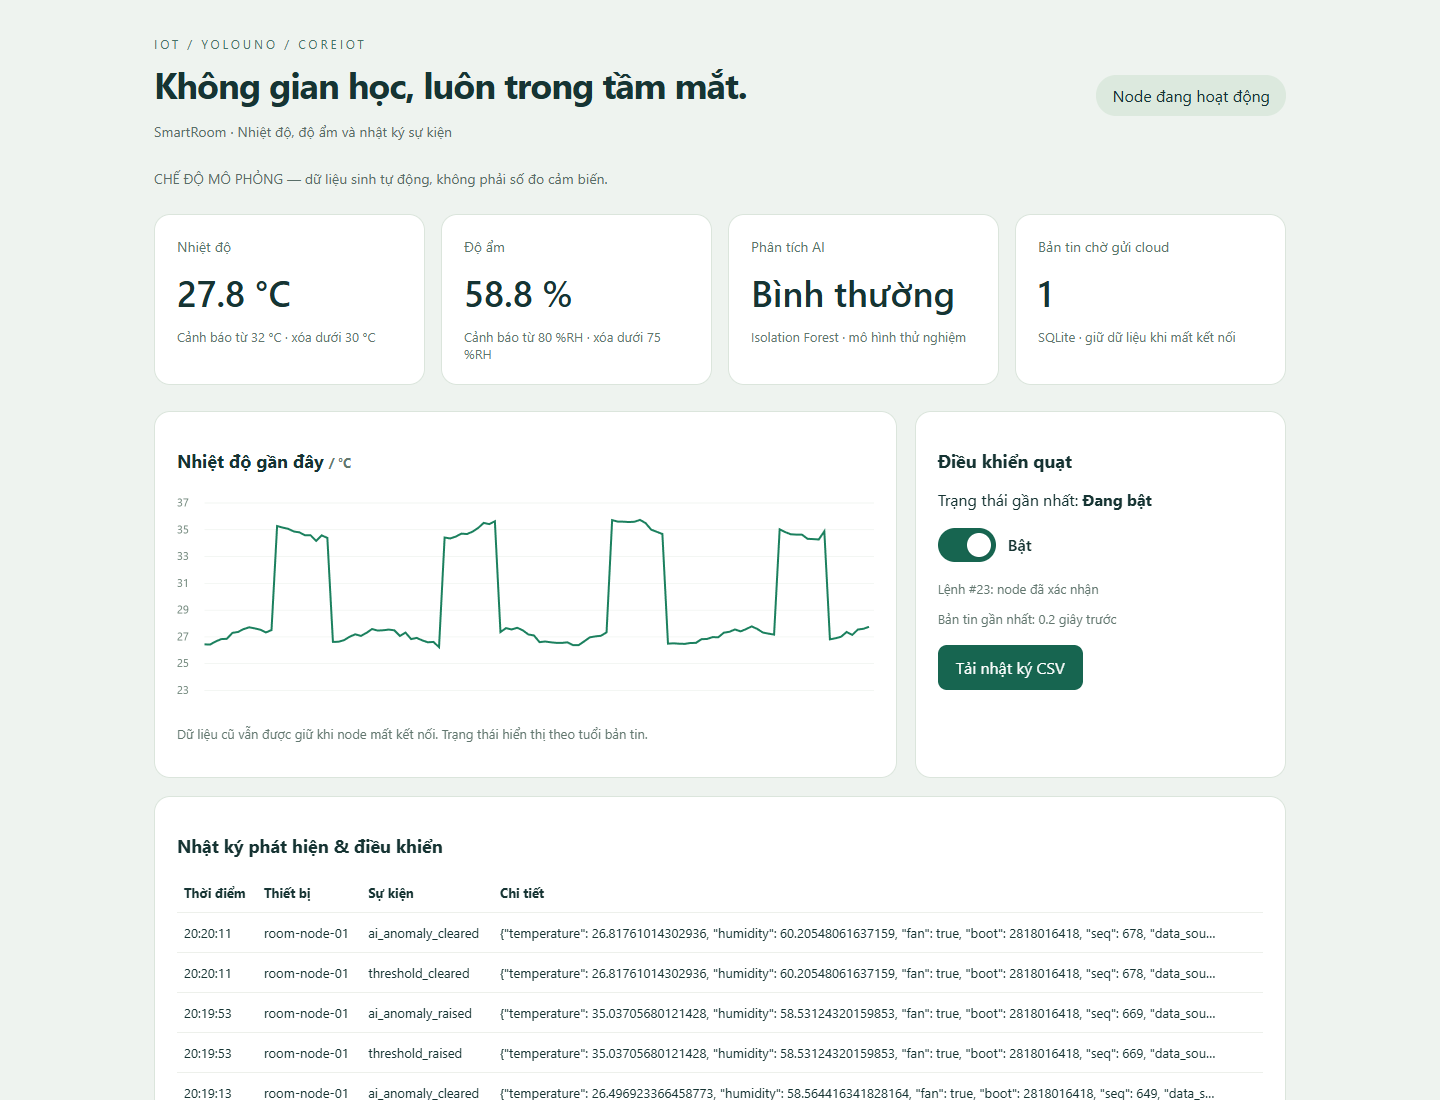
\includegraphics[width=\textwidth,height=.70\textheight,keepaspectratio]{../evidence/dashboard_current_desktop.png}
\caption{Ảnh Chrome ngày 26/11 của gateway đang chạy tại cổng 8081: switch quạt và AI đã nạp model; nguồn sensor mô phỏng. Chụp chỉ đọc, không gửi lệnh trong lượt chụp.}
\end{figure}
Nhật ký được ghi SQLite và xuất CSV toàn bộ events qua \code{/api/events.csv}. Hiển thị bảng dùng \code{textContent} để dữ liệu không bị thực thi như HTML. API điều khiển kiểm tra Origin cùng Host khi trình duyệt cung cấp; mặc định loopback hạn chế truy cập mạng ngoài. Phiên bản hiện tại chưa có tài khoản người dùng, reverse proxy HTTPS hoặc phân quyền nhiều người, nên không mở trực tiếp cổng này ra Internet.

\section{Trí tuệ nhân tạo trên gateway (T09)}
\subsection{Thu thập và chuẩn bị dữ liệu}
\code{ai/train.py} có hai chế độ. Chế độ mặc định sinh 1.500 mẫu bình thường để train; tập test độc lập gồm 800 bình thường, 200 nóng và 200 ẩm cao, tổng 1.200. Bộ sinh dùng seed 2353007. Mẫu bình thường có phân bố quanh 27~°C và 60~\%RH; các tình huống nóng/ẩm được đặt phân bố khác để kiểm tra pipeline. Vì những tình huống này tách khá rõ, accuracy cao không phải bằng chứng về độ khó thực tế.

Chế độ CSV yêu cầu cột \code{temperature,humidity,label}, nhãn 0/1 và thứ tự thời gian. 60\% đầu là miền train, chỉ lấy mẫu normal trong phần này; 40\% cuối dành cho test. Cần ít nhất 100 mẫu normal train và 50 mẫu test hữu hạn có đủ hai lớp. Khi thu thập thực tế, phải ghi bối cảnh, phiên/phòng và cách gán nhãn; không tự tạo nhãn bằng đúng luật ngưỡng rồi dùng kết quả để khẳng định AI vượt luật đó.

Bản cập nhật kiểm tra toàn bộ CSV trước khi chia tập: đủ cột; nhãn đúng 0 hoặc 1, không làm tròn nhãn thập phân; nhiệt độ hữu hạn trong $[-40,85]$ và độ ẩm trong $[0,100]$. Miền này khớp hàng rào dữ liệu gateway, không phải chứng nhận cảm biến. Thứ tự thời gian vẫn do người cung cấp CSV đảm bảo vì định dạng hiện không bắt buộc cột timestamp.

\subsection{Huấn luyện và đánh giá}
Isolation Forest gồm 100 cây, contamination 0,02, random state cố định và chạy CPU một job. Không có bước chọn hyperparameter dựa trên tập test. Mô hình trả decision score; giá trị âm được đánh dấu anomaly. Tài liệu thư viện mô tả tham số và quy ước score này \cite{isolation}.

Các chỉ số tính trên tập test độc lập là precision, recall, F1 và accuracy. Với lớp bất thường, đặt TP là phát hiện đúng, FP là báo động giả, FN là bỏ sót:
\[
P=\frac{TP}{TP+FP},\qquad R=\frac{TP}{TP+FN},\qquad
F_1=\frac{2PR}{P+R}.
\]
Số liệu cụ thể và confusion matrix nằm ở Chương 4; file CSV lưu từng dự đoán để tái kiểm tra. Tách đánh giá AI khỏi đánh giá ngưỡng tránh đồng nhất hai cơ chế.

Module \code{ai/evaluate.py} nạp model cố định, kiểm tra SHA-256 và so sánh với luật ngưỡng nhiệt độ $\geq32$ hoặc độ ẩm $\geq80$. Luật so sánh từng mẫu không có hysteresis; hysteresis của ứng dụng đã được kiểm tra bằng chuỗi riêng. Đánh giá gồm bộ gốc, năm seed mới cùng phân bố, trường hợp normal dịch phân bố, lạnh chưa có trong tập huấn luyện và bất thường hiếm. Không huấn luyện lại, tìm ngưỡng hoặc đổi contamination sau khi xem kết quả. Nhãn do kịch bản sinh dữ liệu quy định, không phải số đo thực. Decision score không phải xác suất tin cậy; không đổi score thành phần trăm chính xác.

\subsection{Triển khai mô hình}
Model được xuất \code{ai/model.joblib} và nạp một lần khi gateway khởi động. Mỗi mẫu hợp lệ được bổ sung \code{anomaly_score}, \code{anomaly}, \code{inference_ms} và \code{ai_available}. Nếu chưa có model, giao diện hiển thị chưa có model; không gán nhãn ``bình thường'' giả. Model đặt trên PC, không đưa lên ESP32 nên không đăng ký TinyML.

Khi thay dữ liệu hoặc phiên bản scikit-learn, nên train lại và khởi động lại gateway. Chỉ nạp model do nhóm tự tạo hoặc từ nguồn tin cậy. Bản model sinh phục vụ demo có thể khác rõ dữ liệu phòng học thật, vì vậy cần một giai đoạn thu dữ liệu trước khi dùng score làm cơ sở vận hành.

\section{Nền tảng CoreIOT}
\subsection{Device Profile, template và dashboard (T11)}
Nhóm sử dụng cổng web \url{https://app.coreiot.io/home}. Các ảnh và cấu hình thực đã được lưu trong \code{evidence/coreiot/}. Export \code{smartroom_co3037.json} có bốn widget: Temperature, Humidity, bảng Alarms và Single Switch Fan. Alias cảm biến tìm \code{room-node-01}; switch chọn cùng hệ thống thiết bị và lấy time-series \code{fan}. API local trước đó ghi nguồn \code{simulation}, RPC ID applied và outbox bằng 0. MQTT dùng \code{app.coreiot.io:1883} theo tài liệu CoreIOT \cite{coreiotconnect}.

\begin{figure}[H]\centering
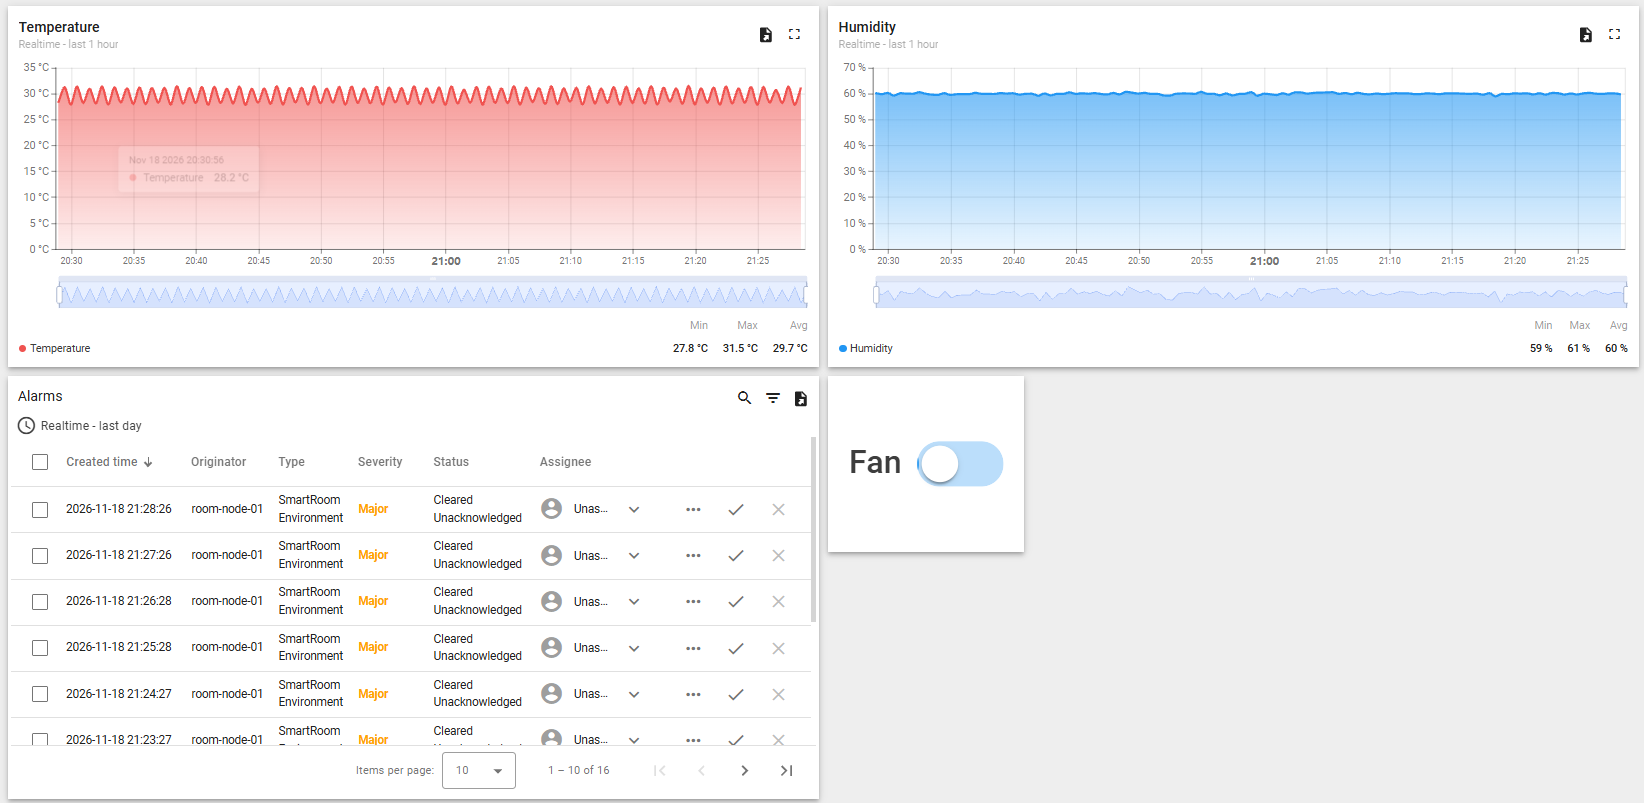
\includegraphics[width=\textwidth,height=.58\textheight,keepaspectratio]{../evidence/coreiot/SmartRoom_Dashboard.png}
\caption{Ảnh CoreIOT gốc lưu ngày 18/11: hai biểu đồ, Single Switch Fan và alarm; chưa có các thẻ AI bổ sung ngày 26/11. Nguồn cảm biến mô phỏng.}
\label{fig:coreiot-dashboard}
\end{figure}

\code{coreiot/smartroom_dashboard.json} giữ hai time-series widget và alarm table từ template Thermostats chính thức. File nguồn, commit SHA, SHA-256 và giấy phép Apache-2.0 được lưu trong \code{coreiot/templates/}. Dự án thay alias thành \code{room-node-01}, bố cục và nhãn; bỏ map và form quản trị không phục vụ đề tài. Phần giao diện widget kế thừa không được trình bày như mã hoàn toàn do nhóm viết.

Ảnh và export gốc xác nhận trục Humidity dùng đơn vị \%. Bản ngày 18/11 còn AVG mỗi 30 giây; bản mới \code{smartroom_dashboard_20261126.json} đã xác nhận cả hai biểu đồ dùng aggregation NONE, cửa sổ riêng 1 giờ. Các đỉnh ngắn được hiển thị bằng dữ liệu gốc; RuleChain vẫn xét telemetry đầu vào. Hai bản export được giữ riêng theo ngày, không sửa cấu hình cũ để giả như thay đổi đã có trước đó.

Bản \code{coreiot/smartroom_dashboard_rpc.json} trước đây được dùng khởi tạo hai RPC Button đặt method \code{setFan}, params boolean true/false và target alias sensor. Lệnh dùng two-way, timeout 10 giây; người dùng đã xác nhận vận hành và gateway ghi trạng thái applied cho các RPC ID. File này được giữ làm cấu hình ban đầu và fixture kiểm thử, không yêu cầu import lại khi đã có dashboard đang dùng.

Export xác nhận widget \code{system.single_switch} có Initial state=GET\_TIME\_SERIES, key \code{fan}; On/Off đều EXECUTE\_RPC, method \code{setFan}, tham số boolean true/false. Không có lời gọi getFan ở bước lấy trạng thái. Người dùng xác nhận RPC chạy và API local có command applied; chưa dùng ảnh động tác gạt thay cho phản hồi node. Người dùng sửa thủ công nên công cụ REST/DPAPI chỉ là tùy chọn. Dashboard export không chứa runtime ID; URL đang dùng cần đối chiếu riêng, không suy ra từ tiêu đề.

\subsubsection{Các thẻ AI bổ sung ngày 26/11/2026}
Sau khi đánh giá AI và sửa đồng bộ switch, nhóm bổ sung các thẻ quan sát trực tiếp kết quả phân tích trên CoreIOT. Người dùng cung cấp ảnh và xác nhận hoàn tất cấu hình trong trao đổi. Tất cả đọc child \code{room-node-01}; Status widget lấy trạng thái bằng \emph{Get time series}, không gọi RPC để lấy trạng thái model. Các tiêu đề dùng tiếng Anh để thống nhất giao diện.

\begin{longtable}{P{3.3cm}P{3.6cm}P{7cm}}
\caption{Các thẻ trên dashboard sau khi bổ sung AI}\label{tab:coreiot-ai-cards}\\
\toprule Tiêu đề & Widget / key & Ý nghĩa hiển thị \\ \midrule
AI Availability & Status widget; \code{ai_available} & True: MODEL READY; false: MODEL UNAVAILABLE. Xác nhận model đã nạp, không phải độ chính xác của AI. \\
Anomaly Score & Value card; \code{anomaly_score} & Score 4 chữ số thập phân, không có đơn vị; giá trị âm được model đánh dấu bất thường. \\
Anomaly Detection & Status widget; \code{anomaly} & Cờ true: ANOMALY, nền đỏ; false: NORMAL, nền xanh. Export dùng điều kiện On khi kết quả bằng false. \\
Inference Time & Value card; \code{inference_ms} & Thời gian suy luận trên PC, đơn vị ms; không phải độ trễ sensor--cloud. \\
Data Source & Value card; \code{data_source} & Hiện simulation để nhận biết dữ liệu sinh; hardware chỉ khi thật sự chạy từ bridge. \\
Fan & Single Switch; \code{fan} & Đọc trạng thái fan và gửi \code{setFan} boolean; đồng bộ hai chiều đã kiểm tra với node mô phỏng. \\
\bottomrule
\end{longtable}

Ảnh mới đã lưu hiển thị MODEL READY, score 0,2435, NORMAL, inference 6~ms và nguồn simulation; score không âm khớp với trạng thái NORMAL. Hai biểu đồ hiển thị nhiệt độ khoảng 26,1--35,9~°C và độ ẩm 56--64\% trong cửa sổ đang xem; bảng Alarms có các bản ghi SmartRoom Environment đã clear. Biểu tượng score đã đổi từ tam giác cảnh báo đỏ cố định sang biểu tượng thông tin xanh để tránh làm người xem hiểu nhầm mọi score đều là cảnh báo. Đây là một quan sát giao diện, không phải benchmark hoặc phép đo lặp. Người dùng xác nhận đã sửa On/Off; ảnh lưu trực tiếp thể hiện trạng thái normal, chưa là minh chứng riêng cho mọi lần chuyển trạng thái.

Nội dung quan sát, kích thước và SHA-256 ảnh/export mới được ghi tại \code{evidence/coreiot/dashboard_ai_user_check.json}. Hình \ref{fig:coreiot-dashboard} giữ ảnh gốc ngày 18/11; ảnh và JSON ngày 26/11 được lưu riêng. Export mới có 9 widget: 2 biểu đồ, bảng Alarms, Fan, 3 Value card và 2 Status widget. Kiểm tra tĩnh đạt 15/15 điều kiện, gồm layout hợp lệ, hai biểu đồ NONE, các key AI và RPC boolean; kết quả ở \code{evidence/coreiot_dashboard_ai_check.json}.

Riêng Anomaly Detection, \code{compareToValue=false} làm cờ anomaly=false chọn bộ On với chữ Normal/nền xanh; anomaly=true chọn bộ Off với chữ Anomaly/nền đỏ. Đây là ánh xạ hợp lệ đã được đối chiếu trên JSON, không đổi ý nghĩa cờ AI. AI Availability dùng \code{compareToValue=true}, On là Model ready và Off là Model Unavailable. Ba Value card có type latest, lần lượt đọc score, inference và nguồn dữ liệu; score dùng 4 chữ số thập phân, inference có đơn vị ms và 2 chữ số. Giá trị trên thẻ là telemetry gần nhất: khi đánh giá hoạt động cần kiểm tra thời gian cập nhật, không chỉ nhìn chữ MODEL READY.

\IfFileExists{../evidence/coreiot/SmartRoom_Dashboard_20261126.png}{%
\begin{figure}[H]\centering
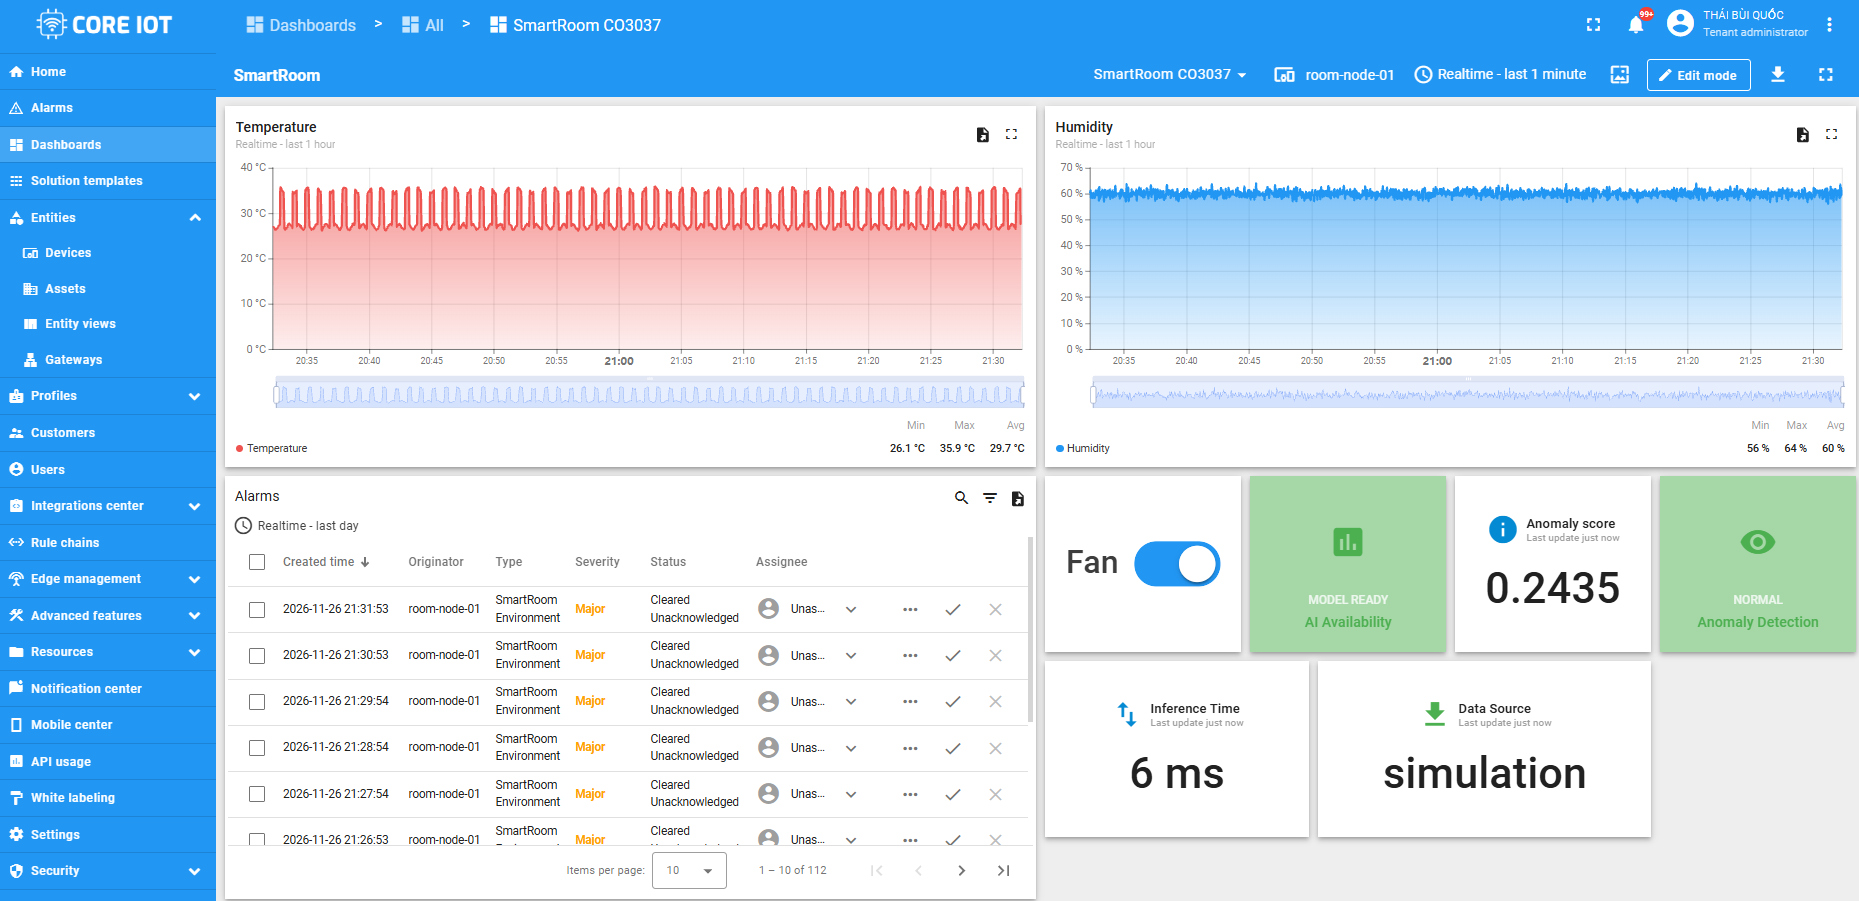
\includegraphics[width=\textwidth,height=.68\textheight,keepaspectratio]{../evidence/coreiot/SmartRoom_Dashboard_20261126.png}
\caption{Dashboard CoreIOT bổ sung các thẻ AI; ảnh người dùng lưu ngày 26/11, nguồn dữ liệu mô phỏng.}
\label{fig:coreiot-dashboard-updated}
\end{figure}
}{%
Ảnh mới đã được xem trong trao đổi nhưng chưa có file gốc tại đường dẫn minh chứng khi dựng PDF. Nhóm cần lưu \code{evidence/coreiot/SmartRoom_Dashboard_20261126.png} để ảnh được tự động nhúng ở lần dựng tiếp theo; bảng cấu hình và quan sát ở trên được giữ rõ nguồn.
}

\subsection{RuleChain và notification (T12, T13)}
RuleChain mới tên \code{SmartRoom alarms}, không đặt làm root toàn tài khoản. Nhánh Post telemetry được lưu timeseries rồi lọc điều kiện nhiệt độ $\geq32$~°C hoặc độ ẩm $\geq80$~\%RH hoặc anomaly=true. Nhánh True tạo alarm type \code{SmartRoom Environment}, mức MAJOR. Nhánh False kiểm tra điều kiện phục hồi: nhiệt độ $\leq30$, độ ẩm $\leq75$ và không anomaly; chỉ khi đạt mới clear. Vùng giữa giữ alarm hiện tại.

Export \code{root_rule_chain.json} xác nhận Post telemetry đi qua bộ lọc \code{metadata.deviceName === "room-node-01"}; True gọi SmartRoom alarms, False lưu timeseries cho các thiết bị khác. Nhánh RPC Request to Device vẫn tới RPC Call Request. Không còn đường lưu telemetry trực tiếp trùng lặp cho SmartRoom ở Root.

\begin{figure}[H]\centering
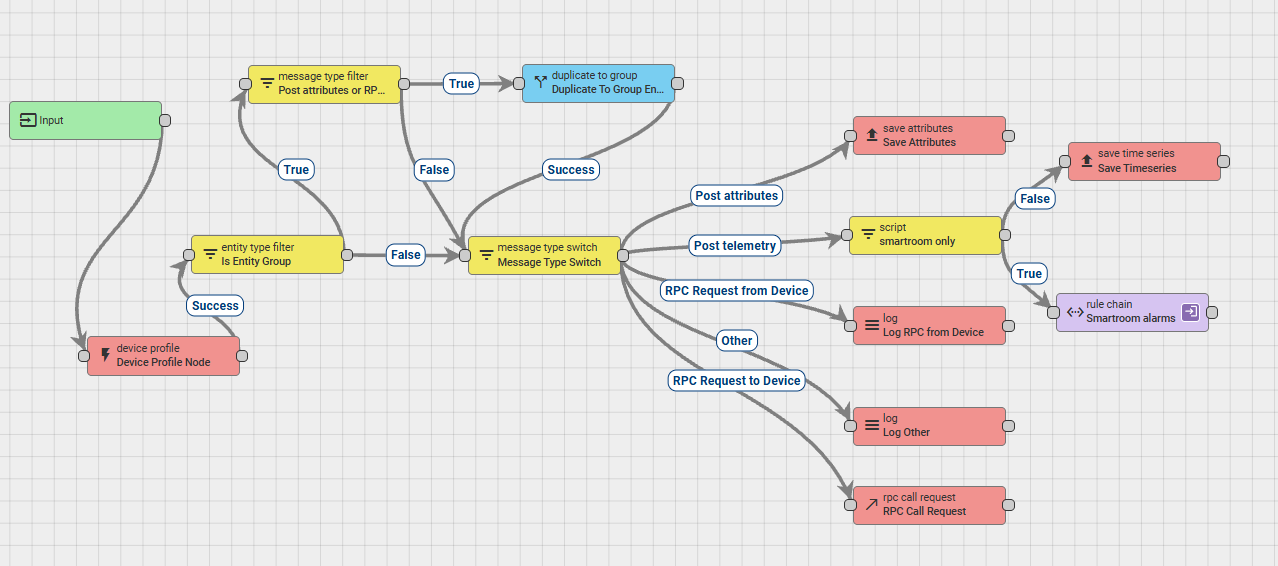
\includegraphics[width=\textwidth,height=.36\textheight,keepaspectratio]{../evidence/coreiot/Rule_chains_root.png}
\caption{Root Rule Chain đã cấu hình trên tài khoản: lọc riêng SmartRoom và giữ đường RPC.}
\label{fig:coreiot-root}
\end{figure}

Export \code{smartroom_alarms.json} xác nhận chuỗi Telemetry only $\rightarrow$ Save timeseries $\rightarrow$ High or anomaly; nhánh True tạo alarm, nhánh False kiểm tra điều kiện phục hồi trước khi clear. Hai action dùng cùng alarm type \code{SmartRoom Environment}; severity tạo là MAJOR.

\begin{figure}[H]\centering
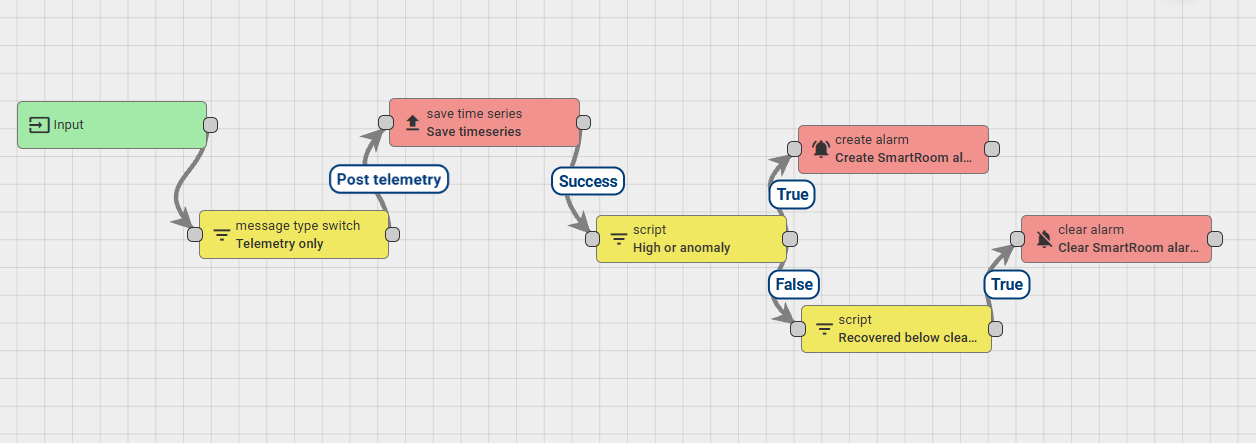
\includegraphics[width=\textwidth,height=.34\textheight,keepaspectratio]{../evidence/coreiot/Rule_chains_SmartRoom_alarms.png}
\caption{SmartRoom alarms thực: tạo alarm và clear với điều kiện phục hồi có hysteresis.}
\label{fig:coreiot-alarms}
\end{figure}

Ảnh dashboard ghi các alarm Major của \code{room-node-01} đã chuyển Cleared Unacknowledged. Ảnh Notification hiển thị cả New alarm và Alarm cleared qua nhiều đợt dữ liệu mô phỏng, xác nhận tạo, phục hồi và gửi Web notification.

\begin{figure}[H]\centering
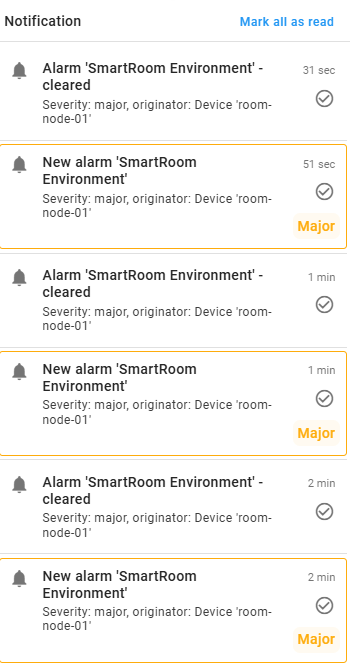
\includegraphics[width=.48\textwidth,height=.63\textheight,keepaspectratio]{../evidence/coreiot/Notification.png}
\caption{Thông báo Web đã nhận cho cả tạo và clear SmartRoom Environment trên CoreIOT.}
\label{fig:coreiot-notifications}
\end{figure}

Thông báo đã có trên tài khoản nên không tạo thêm rule trùng lặp. Chưa có export recipient/template/notification rule nên không khẳng định nhóm tự viết các cấu hình đó. Chưa kiểm chứng email/SMTP. Ảnh gốc và ba JSON export được giữ nguyên; SHA-256 và kết quả kiểm tra nằm ở \code{evidence/coreiot_export_check.json}. Không suy ra độ trễ định lượng từ nhãn thời gian tương đối trên ảnh.

\subsection{Cập nhật OTA (T14)}
Không triển khai. Dự án nạp firmware qua USB bằng PlatformIO; không có phép đo thời gian OTA hoặc phiên bản trước/sau để nhận điểm T14.

\section{Tính năng nâng cao (N06)}
Dashboard riêng không chỉ hiển thị: nó phát hiện chuyển trạng thái threshold/AI, lưu journal bền với thiết bị và timestamp, cho xem lịch sử, xuất CSV và theo dõi lệnh. Sự kiện chỉ ghi khi trạng thái đổi; nhiệt độ lắc quanh 31~°C sau alarm 32~°C không sinh chuỗi cảnh báo/xóa liên tục. Các hành vi này được kiểm thử tự động và quay/chụp trên trình duyệt với node mô phỏng.

N01--N05 và N07 không triển khai. Việc dùng AI để trợ giúp viết code không có nghĩa sản phẩm chứa trợ lý LLM N01. Giao diện responsive được kiểm tra ở chiều rộng 390 px nhưng không gọi là ứng dụng mobile N05.

\chapter{ĐO ĐẠC VÀ KIỂM THỬ HỆ THỐNG}
\section{Môi trường và kịch bản kiểm thử}
Phần mềm được chạy trên Windows 11, Python 3.12.7, NumPy 2.4.4, scikit-learn 1.8.0; mã build dùng PlatformIO 6.2.0. Thời gian đo CPU dùng \code{time.perf_counter()}; lệnh và tuổi bản tin dùng timestamp của PC. Khi chưa có board USB, simulator thay adapter vật lý nhưng vẫn đi qua hàm ingest, command và ack bình thường.

\begin{longtable}{P{1.1cm}P{6.5cm}P{4.2cm}P{2.8cm}}
\caption{Kịch bản và phạm vi bằng chứng}\\
\toprule Mã & Kịch bản & Kết quả mong đợi & Phạm vi \\ \midrule
K01 & Gói hợp lệ, gói trùng, seq cũ và boot mới & Lưu đúng; bỏ trùng; nhận boot mới & Test phần mềm \\
K02 & NaN/Inf, độ ẩm ngoài miền, boolean sai kiểu, device lạ & Từ chối và không tạo reading/outbox & Test phần mềm \\
K03 & 27 $\rightarrow$ 32 $\rightarrow$ 31 $\rightarrow$ 30 °C & Một raised, giữ trạng thái giữa, một cleared & Test phần mềm \\
K04 & Gửi lệnh, ACK sai ID/giá trị rồi ACK đúng & Giữ pending đến ACK đúng & Test phần mềm \\
K05 & Không có ACK, ACK muộn, RPC lặp & Timeout không giả thành công; không áp dụng lặp & Test phần mềm \\
K06 & Publish thất bại và mở lại SQLite & Không mất 1.000 bản tin đã lưu & Benchmark local \\
K07 & HTTP điều khiển, CSV và cross-origin & 202 pending, xuất events, chặn Origin ngoài & Test HTTP thật \\
K08 & Serial chia gói, log boot và JSON sai & Ghép dòng, bỏ sai, nhận local command & Transport giả \\
K09 & Cloud reconnect và RPC đúng payload & Connect child trước telemetry; reply sau ACK & MQTT adapter giả \\
K10 & Chrome desktop/mobile, bật/tắt mô phỏng & Không lỗi JS, không tràn ngang, có applied & Trình duyệt thật \\
K11 & Build hai firmware & Thành công, có file nhị phân và thống kê bộ nhớ & Build thật \\
K12 & Radio, GPIO/quạt và RPC CoreIOT & Đủ ảnh, log, video và số đo lặp & Chưa thực hiện \\
\bottomrule
\end{longtable}

Mỗi test dùng database độc lập; clock giả giúp kiểm tra TTL không cần chờ 5 giây. Việc dùng clock/transport giả không đo thời gian truyền mạng. K09 xác nhận cấu trúc và thứ tự gọi adapter, chưa kiểm tra TLS, SUBACK, quyền tài khoản hay schema của CoreIOT đang dùng.

\section{Kết quả đo}
\subsection{Kiểm thử chức năng và build}
\code{evidence/pytest.xml} ghi \TestCount\ ca kiểm thử, \TestFailures\ lỗi kiểm thử. Log và lệnh thực thi ở \code{evidence/verification.json}. Kiểm tra Chrome điều khiển bật/tắt và chụp màn hình; toàn bộ dữ liệu thiết bị ở lượt đó mang nhãn mô phỏng. Hai firmware đều biên dịch thành công, chưa nạp trên board.

\begin{table}[H]\centering
\caption{Bộ nhớ được trình biên dịch báo cho hai environment}
\begin{tabular}{l r r r}
\toprule Role & RAM tĩnh (byte) & Flash chương trình (byte) & Phân vùng ứng dụng (byte) \\ \midrule
Sensor & 45.392 & 747.613 & 1.310.720 \\
Bridge & 45.344 & 751.573 & 1.310.720 \\
\bottomrule
\end{tabular}
\end{table}
Các con số trên là mức bộ nhớ build, không phải đỉnh heap/stack khi chạy. Chưa có dữ liệu heap dài hạn, nhiệt độ chip hoặc độ ổn định USB.

\subsection{Thời gian xử lý phần mềm}
\code{scripts/evaluate.py} tạo database SQLite tạm trên đĩa, thực hiện 1.000 lần ingest và 100 lần snapshot. Ingest đo kiểm tra + lưu SQLite/outbox, \textbf{không nạp AI} để tách chi phí từng khối. Snapshot đọc trạng thái và 120 mẫu gần nhất. Các mẫu không phải số đo cảm biến; CSV lưu 1.100 thời gian thực đo trên PC.

\begin{table}[H]\centering\small
\caption{Kết quả đo trên PC; đơn vị ms, không phải độ trễ end-to-end}
\begin{tabular}{P{4.6cm}r r r r r}
\toprule Phép đo & Số lần & TB & Nhỏ nhất & Lớn nhất & P95 \\ \midrule
Ingest + commit SQLite & \IngestN & \IngestMean & \IngestMin & \IngestMax & \IngestPNinetyFive \\
Snapshot trạng thái & \SnapshotN & \SnapshotMean & \SnapshotMin & \SnapshotMax & \SnapshotPNinetyFive \\
AI một mẫu trên CPU & \InferenceN & \InferenceMean & \InferenceMin & \InferenceMax & \InferencePNinetyFive \\
\bottomrule
\end{tabular}
\end{table}
\begin{figure}[H]\centering
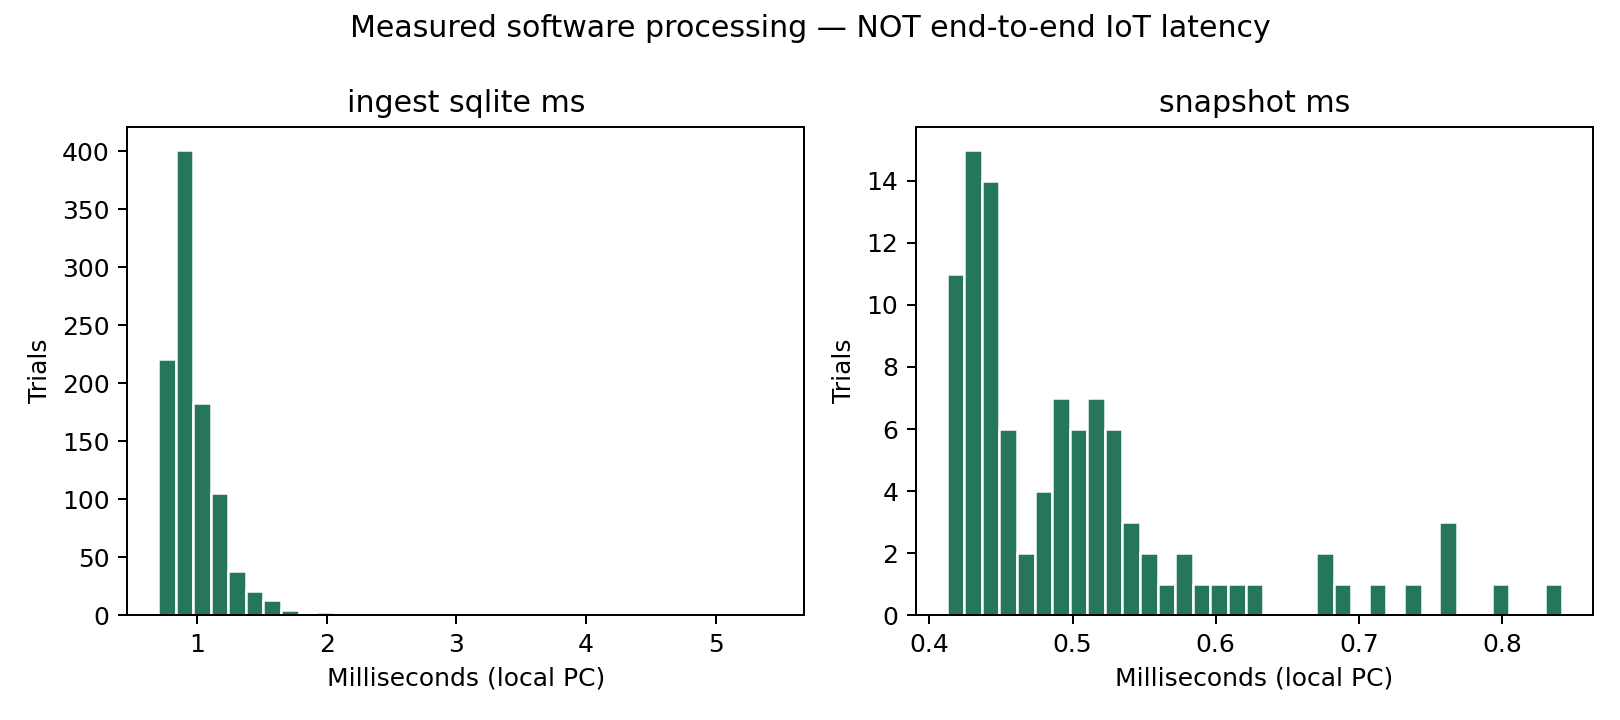
\includegraphics[width=\textwidth]{../evidence/software_latency.png}
\caption{Phân bố thời gian xử lý phần mềm thực đo, chưa bao gồm radio, Internet hoặc CoreIOT.}
\end{figure}
Thời gian thay đổi theo lịch hệ điều hành, I/O và cấu hình máy. Trung bình riêng từng khối không thể cộng để khẳng định độ trễ dashboard dưới một ngưỡng: dashboard poll mỗi giây, và USB, radio, MQTT/cloud đều có độ trễ chưa đo. Snapshot cũng không mô phỏng nhiều người dùng đồng thời.

\subsection{Lưu bền và phục hồi outbox}
Trong lượt đo, số bản tin outbox trước giả lập lỗi publish là 1.000; sau callback publish thất bại vẫn 1.000; đóng/mở database vẫn 1.000. Sau transport giả trả xác nhận thành công, flush được 1.000 và còn 0. Kết quả chứng minh tính lưu bền và điều kiện xóa trong mã local; không chứng minh broker thật đã nhận 1.000 bản tin.

Vì QoS 1 có thể phát lại, timestamp và nội dung gói được giữ; journal không tạo lại khi flush. Chưa kiểm thử mất điện bất ngờ giữa lúc ghi, ổ đĩa đầy, database hỏng hoặc giới hạn lưu trữ nhiều tháng. WAL/giao dịch không thay thế chính sách sao lưu.

\subsection{Đánh giá AI trên dữ liệu sinh}
Huấn luyện dùng \AITrainCount\ mẫu bình thường; tập kiểm thử có \AITestCount\ mẫu độc lập theo seed đã công bố. Accuracy là \AIAccuracy\%; với lớp bất thường, precision \AIPrecision\%, recall \AIRecall\%, F1 = \AIFone. Ma trận nhầm lẫn có TN=\TrueNegative, FP=\FalsePositive, FN=\FalseNegative, TP=\TruePositive.

\begin{figure}[H]\centering
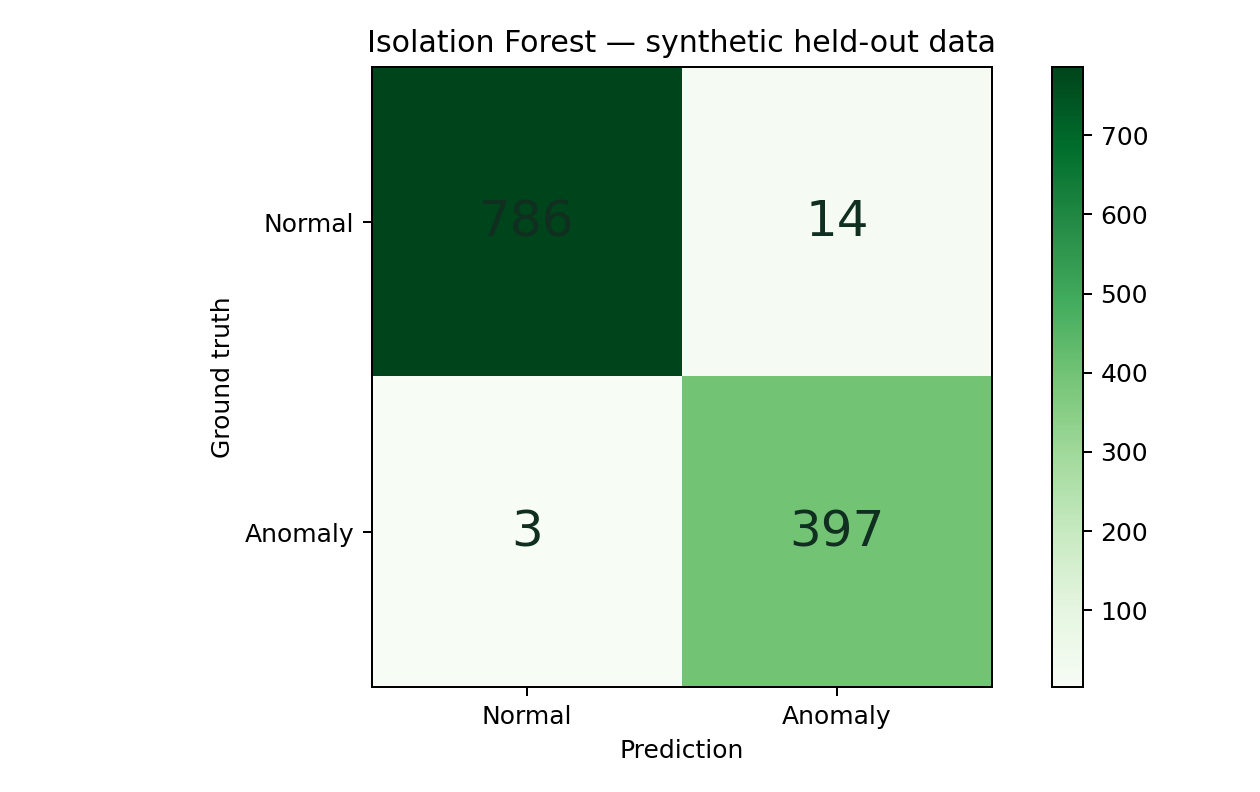
\includegraphics[width=.83\textwidth]{../evidence/confusion_matrix.png}
\caption{Confusion matrix trên dữ liệu sinh giữ riêng; không phải dữ liệu phòng học thực.}
\end{figure}
Những bất thường được sinh cách phân bố bình thường tương đối xa nên mô hình có lợi thế phân tách. Mười bốn báo động giả và ba mẫu bỏ sót trong lượt dữ liệu này cho thấy ngay cả giả thiết đơn giản vẫn có lỗi. Khi dùng phòng thật có thể có thay đổi theo giờ, vị trí cảm biến và nhiều trạng thái hợp lệ chưa có trong train. Cần giữ riêng phiên/ngày/phòng để kiểm tra tổng quát hóa, báo cáo false alarm theo thời gian và xem xét recalibration.

\subsection{Kế hoạch đo phần cứng cần bổ sung}
\begin{longtable}{P{4cm}P{7.2cm}P{3.5cm}}
\caption{Các phép đo thực tế chưa thực hiện, không điền số ước đoán}\\
\toprule Chỉ số & Cách đo và số lần đề xuất & Mục tiêu / trạng thái \\ \midrule
Sensor $\rightarrow$ dashboard & 30 lần; đánh dấu mẫu và sự kiện hiển thị bằng cùng clock/trace hoặc quay màn hình có mốc xác định; nêu rõ chu kỳ lấy mẫu/poll. & $<5$ giây; chưa đo \\
Dashboard $\rightarrow$ ACK & 30 lệnh bật/tắt, lấy thời điểm gửi và nhận ACK cùng PC; thêm quan sát/quay quạt. & $<2$ giây; chưa đo \\
Mất gói ESP-NOW & Theo từng boot, 1.000 gói ở 1/5/10 m; đối chiếu seq gửi và nhận, ghi vật cản/channel. & Ghi trung bình/min/max; chưa đo \\
Tầm truyền & Tăng khoảng cách và ghi tỉ lệ nhận, thời gian thử, môi trường; không chỉ nêu một cự ly duy nhất. & Chưa đo \\
Alert cloud/notification & Ít nhất 10 lần tạo alarm mới; ghi thời điểm phát mẫu, alarm và thông báo nhận. & Chưa đo \\
Độ chính xác cảm biến & So với thiết bị tham chiếu ở nhiều điều kiện; lặp và ghi độ lệch. & Chưa đo \\
Ổn định dài hạn & 24 giờ, ngắt USB/mạng có kịch bản, lưu số reboot và hàng đợi. & Chưa chạy \\
Công suất/OTA & Không có thiết bị đo công suất và không triển khai OTA. & Không báo số liệu \\
\bottomrule
\end{longtable}
Tỷ lệ mất gói theo một phiên có thể tính $100(N_{sent}-N_{received,unique})/N_{sent}$. Cần xác định gói đầu/cuối và số gói sender thật sự gửi, không dùng một khoảng sequence bị cắt đầu/cuối tùy ý. Không trộn nhiều boot hoặc tính gói trùng như gói mới.

\section{Đánh giá kết quả}
Các mục tiêu local về từ chối dữ liệu sai, loại trùng, hysteresis, ACK/timeout và outbox đã có test tương ứng. AI đã có mô hình, phép đo CPU và dữ liệu dự đoán truy xuất được; mức tin cậy hiện giới hạn trong dữ liệu sinh. Hai firmware đủ điều kiện bước tiếp theo là cấu hình MAC/pin và nạp thử, không phải kết luận đã vận hành ổn định.

Telemetry và RPC mô phỏng đã được xác nhận; API local ghi các RPC ID applied và outbox bằng 0. Ảnh người dùng cung cấp còn cho thấy alarm Major, New alarm notification và Alarm cleared notification, xác nhận T12/T13 ở mức chức năng với dữ liệu mô phỏng. Chưa đo lặp độ trễ sensor--cloud, notification hoặc mất gói vô tuyến; không dùng nhãn thời gian tương đối trên ảnh làm số đo độ trễ. Script cập nhật tại chỗ đã kiểm thử cục bộ, nhưng người dùng chọn tự sửa switch. Trước nộp cần lưu tệp ảnh/export cấu hình và thực hiện phép đo phần cứng còn thiếu.

\chapter{KẾT LUẬN VÀ HƯỚNG PHÁT TRIỂN}
\section{Kết quả đạt được}
SmartRoom đã có bộ mã nguồn thống nhất cho hai role ESP32-S3, gateway Python, lưu trữ SQLite, AI trên PC và giao diện local. Các trạng thái quan trọng được biểu diễn tường minh: dữ liệu mới/cũ, alarm raised/cleared và lệnh pending/applied/failed. Bộ đo tạo CSV và biểu đồ từ lần chạy thật trên PC; báo cáo LaTeX được sinh số liệu từ file kết quả để tránh chép lệch.

\begin{table}[H]\centering\small
\caption{Mức hoàn thành theo tính năng ở ngày dựng báo cáo}
\begin{tabular}{P{1cm}P{6.2cm}P{7.2cm}}
\toprule Mã & Đã có & Còn cần thực hiện \\ \midrule
F01 & Firmware đọc/gửi; build hai role & Lắp DHT20, pin/MAC thật, đo radio \\
F02 & SQLite/dashboard/stale và kiểm thử & Chạy từ dữ liệu USB board thật \\
F03 & Journal PC; ảnh/export alarm tạo/xóa và Web notification & Đo độ trễ lặp, chạy dữ liệu cảm biến thực \\
F04 & Model thật; baseline, seed mới, drift và bất thường hiếm & Thu nhãn thực, đánh giá theo phòng/ngày \\
F05 & Switch hai chiều; ACK/TTL và chống lặp theo phiên & Nạp board, quan sát driver/quạt và web bridge \\
F06 & RPC mới applied; dừng/chạy lại khôi phục đồng bộ & Đo reconnect/phát lại có log và thử phần cứng \\
F07 & Ảnh/export cũ; telemetry/switch đang chạy & Thêm ô AI, export lại dashboard và thử thực \\
F08 & Journal/CSV, test, biểu đồ và report & Video demo, timestamp và mã nhóm \\
\bottomrule
\end{tabular}
\end{table}

Những đóng góp kỹ thuật dễ kiểm tra là lưu bền trước khi upload, không xác nhận lệnh chỉ vì đã gửi, chống lặp theo ID, hysteresis giảm dao động cảnh báo và phân biệt rõ dữ liệu sinh với dữ liệu cảm biến. Nhóm chưa dùng bảng này để quy đổi thành điểm đã đạt vì còn thiếu các bằng chứng bắt buộc trên thiết bị và server.

\section{Hạn chế}
Nhóm hiện chưa có mạch nên chưa nạp/chạy board, đo ESP-NOW hoặc có ảnh lắp thật. GPIO/flash cần đối chiếu board lớp. Dashboard, switch hai chiều, RPC, alarm tạo/xóa và Web notification đã có minh chứng với nguồn mô phỏng. Người dùng xác nhận dừng/chạy lại gateway khôi phục đồng bộ, chưa đo thời gian hoặc số bản tin gửi bù. Export cũ còn AVG 30 giây; chưa có export mới để xác nhận aggregation hiện tại. Chưa đo độ trễ lặp, email/SMTP hoặc ổn định dài hạn.

Mô hình AI học dữ liệu sinh và chỉ dùng hai biến tức thời. Luật ngưỡng tốt hơn AI trên các cụm nóng/ẩm đang dùng; AI nhạy với dịch phân bố normal và có precision thấp hơn khi bất thường hiếm. Phát hiện tình huống lạnh khác phân bố là khả năng bổ sung, chưa chứng minh ưu thế với mọi baseline. Chưa có phân tích xu hướng hoặc thích nghi theo mùa/phòng. Hệ thống chưa đo công suất quạt, tốc độ thực hay điều khiển tự động kín vòng.

ID lệnh được lưu bền ở gateway và node; nếu xóa DB mà giữ NVS, ID mới có thể nhỏ hơn ID node nhớ và bị từ chối. Lệnh cũng chỉ có ACK trạng thái firmware, chưa có clock đồng bộ để loại trừ mọi lệnh trễ trong đường truyền. Outbox có giới hạn bản tin nhưng readings/events chưa có retention. Dashboard local chưa có phân quyền đa người dùng; không mở ra Internet.

\section{Hướng phát triển}
Khi chưa có mạch, nhóm có thể hoàn thiện ô AI/score/nguồn dữ liệu trên CoreIOT, lưu export mới và quay demo phần mềm với nhãn mô phỏng. Khi có thiết bị, tiếp tục xác nhận pin, chạy hai board, log seq/ACK, đo độ trễ và bổ sung video thực. Dữ liệu AI cần thu nhiều phiên/phòng, mô tả nhãn độc lập và giữ test tách theo ngày; không điều chỉnh model chỉ để tăng điểm trên bộ sinh hiện tại.

Phiên bản hiện tại đã tách request ID RPC theo phiên MQTT. Bước tiếp theo có thể bổ sung command epoch giữa gateway và node để khôi phục sau thay máy, đồng bộ thời gian phục vụ đo end-to-end, retention/sao lưu DB và kiểm thử 24 giờ. Khi cần tự động điều khiển, nên thêm cảm biến phản hồi quạt và chính sách an toàn độc lập AI. OTA chỉ đăng ký khi có quy trình đóng gói, kiểm tra phiên bản, rollback và minh chứng cập nhật thật; chưa đưa vào điểm hiện tại.

\chapter{HƯỚNG DẪN SỬ DỤNG MÃ NGUỒN}
\section{Repository và cấu trúc thư mục}
Repository: \href{\RepoURL}{github.com/Funacius/smartroom-iot-co3037}. Dự án được tạo riêng tư; trước khi nộp, chủ repository cấp quyền cho tài khoản GitHub do giảng viên cung cấp hoặc tự quyết định chuyển công khai. Không cần công khai token/cấu hình local.
\begin{verbatim}
smartroom-iot-co3037/
  firmware/      platformio.ini, boards/, include/, src/
  gateway/       core.py, transports.py, server.py, dashboard.html
  ai/            train.py, model.joblib
  coreiot/       templates/, rulechain/, JSON, README.md
  tests/         test_gateway.py, test_transports.py
  scripts/       evaluate, verify, build_report, record_hardware
  report/        main.tex, chapters/, metadata.json, PDF
  docs/          DEMO.md, source/
  evidence/      logs, metrics, CSV, charts, screenshots
  README.md
\end{verbatim}
Các đường dẫn trong hướng dẫn được tính từ gốc repository. Thư mục \code{runtime/}, môi trường ảo, \code{.pio/}, token và cấu hình local được bỏ qua bởi Git. Không giả lập commit của từng thành viên; mỗi người tự commit đóng góp thực tế.

\section{Yêu cầu môi trường}
Máy phát triển cần Python 3.12, PlatformIO Core 6.2.0 hoặc extension PlatformIO đã cài trên VS Code, Git và trình duyệt. Phần nạp cần cáp dữ liệu, USB driver tương ứng và quyền mở cổng COM. Dựng báo cáo cần XeLaTeX từ MiKTeX/TeX Live với Times New Roman, Arial và Consolas. Các thư viện Python được liệt kê trong \code{requirements.txt}; phiên bản đã dùng được lưu ở \code{evidence/python_versions.json}.

Tiện ích \href{https://marketplace.visualstudio.com/items?itemName=lxvs.docx-previewer}{Docx Previewer -- lxvs.docx-previewer} đã được cài trên VS Code để mở \code{IoTReport_Template.docx}. Chọn file DOCX; nếu VS Code mở dạng nhị phân, dùng Open With rồi chọn Docx Previewer. Tiện ích dùng để xem, không thay thế toàn bộ khả năng chỉnh sửa Word. VS Code đã có PDF viewer để mở PDF đầu ra.

\section{Cài đặt và cấu hình}
\subsection{Lấy mã và tạo môi trường Python}
\begin{verbatim}
git clone https://github.com/Funacius/smartroom-iot-co3037.git
cd smartroom-iot-co3037
python -m venv .venv
.venv\Scripts\python -m pip install -r requirements.txt
.venv\Scripts\python ai/train.py
\end{verbatim}
Repository riêng tư yêu cầu tài khoản đã được cấp quyền. Lệnh train mặc định sinh dữ liệu có nhãn nguồn, xuất model, metrics, dự đoán từng dòng và confusion matrix. Môi trường khác phiên bản scikit-learn nên train lại trước khi chạy gateway.

\subsection{Cấu hình phần cứng}
Copy \code{firmware/include/config.example.h} thành \code{config.local.h}. Kiểm tra GPIO, logic active-high/low của driver, khóa radio 16 byte, channel, SSID và mật khẩu. Nạp từng role để đọc STA MAC; đặt PEER MAC trên mỗi board thành MAC của board còn lại và nạp lại. File local là cấu hình cho board đang build; phải lưu hai bản riêng ngoài Git hoặc thay đúng MAC khi chuyển role.

Không dùng MAC mẫu cho demo. Flash 4~MB/no PSRAM là cấu hình build bảo thủ của dự án, cần đối chiếu revision thật. Nếu board yêu cầu bootloader mode, dùng BOOT/RESET theo hướng dẫn của thiết bị. Không tự động nạp vào COM3/COM4 Bluetooth chỉ vì các cổng đó xuất hiện.

\subsection{Cấu hình gateway và CoreIOT}
Server lớp là \url{https://app.coreiot.io/home}. Sau đăng nhập, mở Entities $\rightarrow$ Devices, nhấn dấu cộng, tạo \code{smartroom-pc-gateway}, giữ profile mặc định cho lần thử đầu và bật Is gateway. Mở Manage credentials/Copy access token của thiết bị đó. Token là của gateway, không phải token child. Không gửi token trong cuộc trò chuyện.

Chạy \code{python scripts/start_coreiot.py} tại gốc dự án. Chương trình hỏi token kín, tạo \code{runtime/coreiot_config.json} từ profile CoreIOT riêng và mở dashboard mô phỏng tại \code{127.0.0.1:8081}. Profile dùng \code{app.coreiot.io:1883}, không TLS, theo tài liệu CoreIOT; database mô phỏng cloud riêng tránh phát lại lịch sử demo local. Token chỉ truyền qua môi trường tiến trình con, không lưu cấu hình. Sau khi kết nối, tìm child \code{room-node-01} và kiểm tra Latest telemetry với \code{data_source=simulation}. Người dùng đã nhận telemetry và gửi ảnh dashboard cơ bản. Bước tiếp theo là import \code{coreiot/smartroom_dashboard_rpc.json}, kiểm tra đơn vị \% và thử hai nút để xác nhận RPC.

Khi chạy phần cứng, sửa cổng Serial trong runtime config rồi thêm \code{--hardware} cho script. Với endpoint khác có TLS, dùng profile chung \code{gateway/config.example.json} và cổng/chứng chỉ do quản trị cung cấp. Đọc đầy đủ \code{coreiot/README.md} để import dashboard, gắn chain và tạo recipient/template thông báo.

Để nhập token kín trong PowerShell:
\begin{verbatim}
$secret = Read-Host 'Gateway access token' -AsSecureString
$env:COREIOT_TOKEN = [System.Net.NetworkCredential]::new(
  '', $secret).Password
\end{verbatim}
Trong terminal thực, có thể đặt phép gán token trên cùng một dòng như README. Không điền token vào source, report, ảnh chụp hoặc commit. Nếu server chỉ hỗ trợ cổng không TLS, xác nhận cấu hình lớp trước khi đổi mặc định; không tắt kiểm tra chứng chỉ để vượt lỗi hostname/CA.

\section{Build, nạp và chạy}
\subsection{Chạy mô phỏng trước khi có board}
\begin{verbatim}
.venv\Scripts\python -m gateway.main --simulate
\end{verbatim}
Mở \code{http://127.0.0.1:8080}. Trong mỗi vòng 60 giây, có 20 giây bình thường, 20 giây nóng và 20 giây hồi phục. Xem alarm/AI/journal, thử bật/tắt và xuất CSV. Database simulation tách khỏi database hardware. Không có \code{--cloud} thì không kết nối CoreIOT và outbox sẽ tăng. Ctrl+C dừng dịch vụ.

\subsection{Build và nạp firmware}
\begin{verbatim}
pio run -d firmware
pio run -d firmware -e sensor -t upload --upload-port COM5
pio device monitor --port COM5 --baud 115200
pio run -d firmware -e bridge -t upload --upload-port COM6
\end{verbatim}
COM5/COM6 là ví dụ phải thay theo máy. Nếu \code{pio} chưa có trong PATH, dùng terminal PlatformIO hoặc cài CLI vào môi trường Python. Tắt monitor đang giữ cổng bridge trước khi chạy gateway. Sensor phải có cấu hình peer của bridge và ngược lại; cùng channel và key. Cấp nguồn node A, nối USB node B với PC rồi chạy:
\begin{verbatim}
.venv\Scripts\python -m gateway.main --config runtime/config.json
\end{verbatim}
Để thêm cloud, sau khi nhập token và hostname đúng, thêm \code{--cloud}. Có thể dùng \code{--simulate --cloud} để thử API trước; dữ liệu phải giữ nhãn simulation và không dùng làm số đo phần cứng. Khi chạy web bridge, PC vẫn cần gateway để thực hiện yêu cầu điều khiển.

\subsection{Chạy kiểm thử và dựng lại PDF}
\begin{verbatim}
.venv\Scripts\python -m pytest -q --junitxml=evidence/pytest.xml
.venv\Scripts\python scripts/evaluate.py
.venv\Scripts\python scripts/verify.py --firmware
.venv\Scripts\python scripts/build_report.py
\end{verbatim}
Script dựng báo cáo lấy tên, mã nhóm, email và link từ \code{report/metadata.json}; đọc số đo AI/benchmark/JUnit rồi chạy XeLaTeX hai lượt. Khi đã có mã nhóm, thay metadata và dựng lại để tên PDF đúng \code{[ClassCode]_[GroupCode]_IoTReport.pdf}. Ngày trong metadata là ngày báo cáo, cần cập nhật khi nộp.

\subsection{Xử lý lỗi thường gặp}
\begin{longtable}{P{4cm}P{10.8cm}}
\toprule Biểu hiện & Kiểm tra và cách xử lý \\ \midrule
Không có mẫu mới & Đúng COM, monitor đã đóng, cáp dữ liệu, DHT20/pin, MAC/key/channel hai board. Không sửa bằng cách tạo telemetry giả. \\
Web bridge điều khiển không đổi quạt & PC gateway phải chạy; xem pending/failed và Serial ACK. Web bridge không tự cấp command ID. \\
Lệnh luôn timeout sau đổi máy & Kiểm tra DB/NVS command ID. Nếu bắt đầu đợt mới và đã xóa DB, chủ ý đồng bộ/reset NVS node; sao lưu trước. \\
Outbox tăng & Không bật cloud, sai hostname/token/TLS hoặc chưa đăng ký child. Kiểm tra token gateway và quyền server. \\
CoreIOT không hiện dữ liệu & Tên child chính xác, gateway Is gateway, topic Gateway API tương thích; xác minh trên Latest telemetry trước dashboard. \\
Alarm có nhưng không có thông báo & Notification rule/recipient/template và SMTP; alarm table không phải bằng chứng notification. \\
Model không nạp hoặc sai phiên bản & Chạy lại train trong cùng môi trường rồi restart gateway; không nạp model từ nguồn không tin cậy. \\
\bottomrule
\end{longtable}

\begin{thebibliography}{99}
\addcontentsline{toc}{chapter}{Tài liệu tham khảo}
\bibitem{assignment} Trường Đại học Bách khoa -- ĐHQG-HCM, ``Course Project Requirements -- Internet of Things (IoT), Semester 261,'' 27/10/2026. Tệp học phần: \code{Project_Annoucement_IoT.pdf}; kèm \code{IoTReport_Template.docx}.
\bibitem{ohstem} OhStem Education, ``Đo và hiển thị nhiệt độ \& độ ẩm,'' Yolo UNO Smart Home. [Trực tuyến]. \url{https://docs.ohstem.vn/en/latest/yolo_uno/smart_home_uno/dht20.html}. Truy cập: 18/11/2026.
\bibitem{espnow} Espressif Systems, ``ESP-NOW,'' ESP-IDF Programming Guide v4.4.7, ESP32-S3. [Trực tuyến]. \url{https://docs.espressif.com/projects/esp-idf/en/v4.4.7/esp32s3/api-reference/network/esp_now.html}. Truy cập: 18/11/2026.
\bibitem{dht20} R. Tillaart, ``DHT20: Arduino library for DHT20 I2C temperature and humidity sensor.'' [Mã nguồn]. \url{https://github.com/RobTillaart/DHT20}. Bản dùng: 0.3.2. Truy cập: 18/11/2026.
\bibitem{tbtemplate} ThingsBoard Authors, ``Thermostats demo dashboard,'' ThingsBoard source repository, Apache-2.0. [Mã nguồn]. \url{https://github.com/thingsboard/thingsboard/blob/master/application/src/main/data/json/demo/dashboards/thermostats.json}. Bản tải có commit và hash tại \code{coreiot/templates/PROVENANCE.json}. Truy cập: 18/11/2026.
\bibitem{gatewayapi} ThingsBoard Authors, ``Gateway API Overview,'' ``Telemetry,'' và ``RPC.'' [Trực tuyến]. \url{https://thingsboard.io/docs/reference/gateway-api/overview/}; \url{https://thingsboard.io/docs/reference/gateway-api/telemetry/}; \url{https://thingsboard.io/docs/pe/reference/gateway-api/rpc/}. Truy cập: 18/11/2026. Dùng làm cơ sở adapter, chưa xác minh phiên bản CoreIOT của lớp.
\bibitem{isolation} scikit-learn Developers, ``IsolationForest,'' API Reference. [Trực tuyến]. \url{https://scikit-learn.org/stable/modules/generated/sklearn.ensemble.IsolationForest.html}. Môi trường chạy dùng scikit-learn 1.8.0. Truy cập: 18/11/2026.
\bibitem{paho} Eclipse Foundation, ``Paho MQTT Python client.'' [Mã nguồn và tài liệu]. \url{https://github.com/eclipse-paho/paho.mqtt.python}. Dự án dùng Callback API v2. Truy cập: 18/11/2026.
\bibitem{ruleengine} ThingsBoard Authors, ``Rule Engine.'' [Trực tuyến]. \url{https://thingsboard.io/docs/user-guide/rule-engine/}. Truy cập: 18/11/2026.
\bibitem{sqlite} SQLite Authors, ``Write-Ahead Logging.'' [Trực tuyến]. \url{https://www.sqlite.org/wal.html}. Truy cập: 18/11/2026.
\end{thebibliography}

\appendix
\chapter{MINH CHỨNG, DEMO VÀ KHAI BÁO AI}
\section{Bản đồ minh chứng trong repository}
\begin{longtable}{P{6.1cm}P{8.7cm}}
\toprule Đường dẫn & Nội dung và giới hạn \\ \midrule
\code{evidence/pytest.xml}, \code{pytest.log} & Test đã chạy; không thay cho test radio hoặc tài khoản CoreIOT. \\
\code{evidence/firmware_build.log} & Biên dịch hai role, RAM/flash; không chứng minh board đã boot. \\
\code{evidence/software_metrics.json}, \code{software_trials.csv} & 1.100 lần đo xử lý trên PC và kiểm tra outbox. \\
\code{evidence/ai_metrics.json}, \code{ai_test_predictions.csv} & Dữ liệu sinh có seed; confusion matrix và suy luận CPU. \\
\code{evidence/browser_check.json}, \code{dashboard_desktop.png}, \code{dashboard_mobile.png} & Chrome chạy ứng dụng local với nguồn simulation; không phải ảnh CoreIOT. \\
\code{coreiot/templates/PROVENANCE.json} & Nguồn template, commit, hash, giấy phép và phạm vi sửa. \\
\code{evidence/coreiot_progress.json} & Xác nhận của người dùng về Latest telemetry và snapshot trạng thái gateway local; chưa có ảnh cloud hoặc kiểm chứng RPC. \\
\code{docs/DEMO.md} & Kịch bản và câu hỏi bảo vệ; chưa phải video đã quay. \\
\code{evidence/hardware/} & Nơi bổ sung dữ liệu/ảnh thực. Hiện chưa có minh chứng thiết bị trong phiên dựng mã. \\
\bottomrule
\end{longtable}

\section{Kịch bản video đề xuất}
Video dự kiến 7--9 phút: giới thiệu mạch; cho thấy sequence ESP-NOW; mở web bridge; điều khiển với ACK; xem score AI và journal; xem gateway-child và dashboard CoreIOT; tạo/clear alarm và nhận notification; ngắt mạng và nối lại; xem stale khi sensor mất; cuối cùng đối chiếu bảng tự đánh giá. Mốc thời gian trong \code{docs/DEMO.md} chỉ là kế hoạch. Khi đã quay, nhóm thay bằng timestamp thật và điền link vào metadata.

Mỗi mục đăng ký điểm cần liên kết trực tiếp với đoạn demo, screenshot hoặc log tương ứng. Mã nhóm và ngày nộp cũng cần cập nhật theo LMS. Commit history phải phản ánh đóng góp thực tế của hai người; không sửa author để tạo cảm giác mỗi thành viên đã tự làm phần chưa thực hiện.

\section{Khai báo phạm vi sử dụng công cụ AI}
Trong phiên làm việc này, công cụ AI hỗ trợ đọc đề bài/mẫu, chọn đề tài, đề xuất kiến trúc, viết firmware/gateway/dashboard/test, tạo script dữ liệu và soạn LaTeX. Công cụ cũng chạy các kiểm thử và phép đo được ghi log trên máy tính. Những kết quả đó phải được thành viên nhóm đọc, hiểu, thực thi lại và xác minh trước khi nộp.

AI không cung cấp số đo cảm biến thực, ảnh lắp mạch, video demo hay thông báo CoreIOT giả. Tại thời điểm dựng báo cáo, chưa nạp board hoặc đo ESP-NOW; người dùng tự cấu hình tài khoản CoreIOT và xác nhận đã thấy telemetry mô phỏng. AI đọc trạng thái gateway local nhưng chưa trực tiếp quan sát tài khoản cloud hoặc thử RPC từ cloud. Bảng phân công là đề xuất; không trình bày mã sinh trong phiên này như lịch sử đóng góp thủ công đã hoàn tất của hai thành viên.

Phần tái sử dụng gồm thư viện Arduino/ESP-IDF, DHT20, ArduinoJson, Paho, scikit-learn và widget template ThingsBoard. Phần điều phối packet/ACK/outbox, dashboard HTML local, kịch bản test/đo và văn bản báo cáo được xây dựng cho dự án với trợ giúp AI. Mỗi thành viên chịu trách nhiệm giải thích phần được phân công khi vấn đáp.
\section{Checklist trước nộp}
\begin{enumerate}
\item Xác nhận mã lớp và mã nhóm; đổi tên PDF theo quy định.
\item Nạp/chạy hai board, xác nhận pin/nguồn/MAC/key/channel; lưu ảnh mạch thật.
\item Đo các kịch bản còn thiếu với số lần lặp, mean/min/max và dữ liệu gốc.
\item Kết nối CoreIOT, import/export cấu hình thật và nhận notification thật.
\item Cập nhật tự đánh giá theo bằng chứng, không tự nhận T01/T04/T05/T14/N07.
\item Quay video và điền link; cấp quyền GitHub cho giảng viên.
\item Hai thành viên tự commit phần công việc thực tế, hoàn chỉnh phân công và dựng lại PDF.
\end{enumerate}

\end{document}
